%\sorgt 	%ensures the apparition of "Appendix" before each appendix.
%\openany	%ensures that a chapter can begin on each side and not only on the right site.
%\bibtotoc	%ensures that the bibliography automatically appears in the table of contents.
%\documentclass[colordvi,11pt,a4paper,halfparskip,final,headings,appendixprefix,bibtotoc]{scrbook}
\documentclass[
	pdftex,
	chapterprefix,
	headsepline,
	footsepline,
	% colordvi,
	11pt,
	a4paper,
	parskip=half,
	final,
	appendixprefix,
bibliography=totoc]{scrbook}

% uncomment the following line (mutual exclusive to the one above) to enter the draft mode.
%\documentclass[colordvi,11pt,a4paper,halfparskip,draft,appendixprefix,bibtotoc]{scrbook}

\newcommand{\studentFirsName}{First Name}
\newcommand{\studentSecondName}{Second Name}
\newcommand{\studentMatrikelnummer}{123456}

% Define a new one if is possible to choose between PDF and DVI.
\usepackage{ifpdf}
\ifx\pdfoutput\undefined
\pdffalse %not PDFLaTeX
\else
\pdfoutput=1
\pdftrue
\fi
%\tracingstats=2
%\usepackage{layout}
% english/spanish/new german language support (hyphenation etc)
\usepackage[english,spanish,ngerman]{babel}

% for prettier tables
\usepackage{booktabs}

% support for latin1 characters. That means you can enter umlauts directly
% no need for "a "u "o "s anymore
\usepackage[ansinew]{inputenc}
%\usepackage[latin1]{inputenc}

% provides the \url{} command to pretty print urls
\usepackage{url}

% needed for a german bibliography-style (s. below)
\usepackage{bibgerm}

% allows text flowing around figures.
\usepackage{wrapfig}

% allows to \includegraphics
\usepackage{graphicx}

% defines some standard colornames like "black" etc.
\usepackage{color}

% allows to color tablecells
\usepackage{colortbl}

% provides an easier interface to if-then-else constructs in 
% custom macros
\usepackage{ifthen}

% allows tables to break over pages.
\usepackage{supertabular}

% allows to have different kinds paper orientations in the same pdf-documnent
\usepackage{pdflscape}

% allows to specify absolute texpos for textboxes. This is generally only important for the titlepage
\usepackage[absolute]{textpos}

% allows to enumerate different figures with a) b) in the same figure-environment.
\usepackage{subfigure}

% finetune the gaps between figure and text in the subfigure environment (basically close the gap as much as possible)
\renewcommand{\subfigtopskip}{0pt}
\renewcommand{\subfigbottomskip}{0pt}

% some color definitions for the pdf statements below
\definecolor{mygrey}{rgb}{0.45,0.45,0.45}
\definecolor{mydarkgrey}{rgb}{0.2,0.2,0.2}
\definecolor{red}{rgb}{1.0,0.33,0.33}
\definecolor{orange}{rgb}{1.00,0.73,0.33}
\definecolor{yellow}{rgb}{0.95,0.92,0.}
\definecolor{lightgreen}{rgb}{0.3,0.95,0.46}
\definecolor{titleblue}{rgb}{0.03,0.10,0.46}

\ifpdf
% Metadata and configuration of the pdf output:
% Do not forget to enter the correct title, author, subject und keywords

% For screen viewing it is nice to have references marked in a slightly different
% color than the rest of the text. Since they will be hyperlinks to the 
% referenced objects.
\usepackage[pdftex,
             pdftitle={},
             colorlinks,
             linkcolor={mydarkgrey},
             citecolor={mygrey},
             urlcolor={black},
             plainpages={false},
             bookmarksnumbered={true},
             pdfauthor={},
             pdfsubject={},
             pdfkeywords={},
             pdfstartview={FitBH}]{hyperref}

% For the final printouts (remember - you need at least three - one for each examiner and one for the archive 
% [ This might have changed - so contact the "Pr�fungsamt" about the current regulations !! ] - it is better
% to have all text in the same color (namely black).
% 
%\usepackage[pdftex,
%            pdftitle={},
%            colorlinks,
%            linkcolor={black},
%            citecolor={black},
%            urlcolor={black},
%            plainpages={false},
%            bookmarksnumbered={true},
%            pdfauthor={},
%            pdfsubject={},
%            pdfkeywords={},
%            pdfstartview={FitBH}]{hyperref}
\pdfcompresslevel=9
\fi

% some configuration for the amount of text on a single page
\usepackage{typearea}
\areaset[1.5cm]{418pt}{658pt}
\setlength{\headheight}{37pt}

% Enter author and title for the titlepage.
\author{}
\title{}

% To avoid nasty mistakes like having comments directly in the textflow
% the following \todo macro was defined. With that you can enter
% \todo{What I still have to do here} 
% inside of your text and a marker will appear at the page's margin with the 
% text "What I still have to do here".
% The first line activates this feature. If you comment it out and uncomment
% the second line below there will be no error messages and no todos will be shown
% anymore. So - even if you have forgotten to delete one of them - they will not appear
% in the final printout. 
\newcommand{\todo}[1]{\marginpar{\textcolor{red}{ToDo:} #1}}
%\newcommand{\todo}[1]{}

% We recommend to split your document into several files. Usually one for every chapter is a 
% good idea. If you follow this guideline (how to assemble these files in a single document
% see two paragraphs below) you will be able to single out chapters via the \includeonly{}
% command. Using this mechanism page numbering and references of the full run before will be
% preserved. This also nice, if your latex run tends to get slow and you need to fine tune 
% some formatting in one chapter - just include that one. The rest (or at least the ones before
% the one currently under construction) will remain untouched. This means a boost in compilation time.
%\includeonly{chapter2}

\begin{document}
% the next two lines influence the detailedness of the table of contents
% and to what structure depth numbers are written before sections/subsections/paragraphs
% You should not touch this
\setcounter{tocdepth}{2}
\setcounter{secnumdepth}{3}
\frontmatter
% here the titlepage is included. Look into the file "titlePage.tex" to 
% adapt it to your needs (name, title etc.)
% Titelseite braucht folgenden  Eintrag
% \usepackage[absolute]{textpos}
% textpos ist nicht Bestandteil von tetex
% kann aber von dante heruntergeladen werden
\begin{titlepage}
\vspace*{-1cm}
\newlength{\links}
\setlength{\links}{0.9cm}
\setlength{\TPHorizModule}{1cm}
\setlength{\TPVertModule}{1cm}
\textblockorigin{0pt}{0pt}

\sf
\LARGE

\begin{textblock}{16.5}(2.8,2.6)
 \hspace*{-0.25cm} \textbf{UNIVERSITÄT DUISBURG-ESSEN} \\
 \hspace*{-1.15cm} \rule{5mm}{5mm} \hspace*{0.05cm} FAKULTÄT FÜR WIRTSCHAFTSWISSENSCHAFTEN\\
 \large{}INSTITUT FÜR INFORMATIK UND WIRTSCHAFTSINFORMATIK \\
 \large{}LEHRSTUHL FÜR PERVASIVE COMPUTING\\
\end{textblock}


%Hier Titel, Name, und Matrikelnummer eintragen, \\ make a newline
\begin{textblock}{14.5}(3.2,8.5)
  \large
{ \bf Bachelor Thesis} \\[1cm]
{\LARGE \Large\bf Design and Implementation of a Distributed, Low-Power, Signal Strength Measurement System} \\[1.3cm]
%APPLICATION OF RADIO TOMOGRAPHIC IMAGING TO SPARSE SYSTEMS DEPLOYED IN INDOOR ENVIRONMENTS
\studentFirsName { } \studentSecondName\\
Matriculation number: \studentMatrikelnummer
\end{textblock}



\begin{textblock}{10}(10.5,17.5)
%
\includegraphics[scale=1.0]{unilogo.pdf}\\

\includegraphics[scale=0.23	]{content/images/NES_Logo.pdf}\\
\normalsize
\raggedleft
Networked Embedded Systems Group \\
Institut für Informatik und Wirtschaftsinformatik \\
Fakultät für Wirtschaftswissenschaften \\
Universität Duisburg-Essen \\[2ex]

\today\\[15ex]
\raggedright
% Prüfers
{\bf First examiner:} Prof. Dr. Pedro José Marrón \\
{\bf Second examiner:} Prof. Dr. Torben Weis \\
{\bf Timespan:} 18. November 2016 - 10. February 2017\\
\end{textblock}


\end{titlepage}

\tableofcontents

%\listoffigures
\mainmatter

% To assemble the whole document
% Please be aware that each file will begin on a new page
% therefore chapters should be put into such a file.
% There cannot be an include statement inside of an "included" file.
% So if you want to further divide your document - use \input inside of 
% the included files. \input will not begin on a new page.
%\setcounter{page}{2}

\cleardoublepage

\section*{Abstract}

%The function of the abstract is to summarize, in one or two paragraphs, the %major aspects of the entire bachelor or master thesis. It is usually written %after writing most of the chapters.

%It should include the following:
%\begin{itemize}
%	\item Definition of the problem (the question(s) that you want to answer) %and its purpose (Introduction).
%	\item Methods used and experiments designed to solve it. Try to describe it %basically, without covering too many details.
%	\item Quantitative results or conclusions. Talk about the final results in a %general way and how they can solve the problem (how they answer the %question(s)). 
%\end{itemize}

%Even if the Title can be a reference of the work's meaning, the Abstract should %help the reader to understand in a quick view, the full meaning of the work. 
%The abstract length should be around 300 words.

%Abstracts are protected under copyright law just as any other form of written %speech is protected. However, publishers of scientific articles invariably make %abstracts publicly available, even when the article itself is protected by a %toll barrier. For example, articles in the biomedical literature are available %publicly from MEDLINE which is accessible through PubMed. It is a common %misconception that the abstracts in MEDLINE provide sufficient information for %medical practitioners, students, scholars and patients[citation needed]. The %abstract can convey the main results and conclusions of a scientific article %but the full text article must be consulted for details of the methodology, the %full experimental results, and a critical discussion of the interpretations and %conclusions. Consulting the abstract alone is inadequate for scholarship and %may lead to inappropriate medical decisions[2].

%An abstract\cite{Ikeda1997, levensthein65:_binar, Middleton2002, salton89} %allows one to sift through copious amounts of papers for ones in which the %researcher can have more confidence that they will be relevant to his research. %Once papers are chosen based on the abstract, they must be read carefully to be %evaluated for relevance. It is commonly surmised that one must not base %reference citations on the abstract alone, but the entire merits of a paper.

Wireless Sensor Networks (WSN) are an emerging technology that enabling new possibilities for localization and tracking. The Radio Tomographic Imaging(RTI) is a localization technique that analyses the signal strength between nodes inside a WSN making it possible to localize and track a person without it carrying a device.

To do this a system that measures the signal strengths of each link inside a WSN is needed. The approaches suggested by the literature however assumes that all the nodes inside a WSN can hear each other, making it impossible to apply this to a WSN that covers large areas like a whole floor or a warehouse.
To make it possible to apply RTI to large environments a new approach that makes signal strength measuring for a WSN possible where not every node can hear all the other nodes is necessary. 

This thesis provides an approach for such a signal strength measurement system that is self calibrating and takes into account that not every node can hear each other, making it possible to deploy it in large areas. To measure the signal strength each node needs to send a message. The suggested approach creates a schedule that defines a predecessor and successor for every node inside the WSN. This makes it possible that the nodes send the messages in a synchronized way avoiding collisions of messages that distort the measurements.

The system is then tested in a WSN with 32 nodes that covers a whole floor of a building with a size of $531 m^2$. These tests show that the the suggested approach can take measurements quick enough to make localization with RTI possible.
\cleardoublepage

\chapter{Introduction}

%[You should answer the question: What is the problem?]

%This paragraph should establish the context of the reported work. To do that, authors discuss over related literature (with citations\todo{how to make %citations}\footnote{To cite a work in latex  }) and summarize the knowledge of the author in the investigated problem.

%An introduction should answer (most of) the following questions:
%\begin{itemize}
%	\item What is the problem that I want to solve?
%	\item Why is it a relevant question?
%	\item What is known before the study?
%	\item How can the study improve the current solutions?
%\end{itemize}

%To write it, use if possible active voice:
%\begin{itemize}
%	\item We are going to watch a film tonight (Active voice).
%	\item A film is going to be watched by us tonight (Passive voice).
%\end{itemize}
%The use of the first person is accepted.

%Rti need to measure the network rss values
%The existing solutions need a single hop network.
%A real deployed network can not necessary depend on this.

%What i wanted to ask you is, how much i need to write inside my motivation and problem description since i do not realy know a lot that can be written %here.
%My idea is to write about the possibility of locating with RTI. Then that this requires a system that sends messages but no two messages at one point in %time.
%Next i would explain that this is solved but only for single hop WSNs. Then give reasons for the use of it in multi-hop WSNs and say that therefore a new %method needs to be developed.
%Then i would explain the requirements for the system and thats basicaly it 


\section{Motivation}

%A good introduction usually starts presenting a general view of the topic and continues focusing on the %%problem studied. Begin it clarifying the subject area of interest and establishing the context (remember %to support it with related bibliography).

%WSN are huge at the momemnt (short explenation, ... make different stuff possible). RTI is one of these uses the rss to localize. needs a system that %sends messages. to provide high accuracy no tow messages are allowed to send at the same time. A approach that does this is needed. for single hop wsns %this is solved via multi spin. in a real world enviroment large areas can not be monitored  since wsn is not single hop.
%New approach that works in multi hop enviroment is required.

Wireless Sensor Networks (WSN) are an emerging technology that enables a lot of different applications for enviromental and habitat monitoring, analysis of structures, or localization and tracking. In the field of localizing and tracking the Radio Tomographic Imaging (RTI) was developed. It is a localization technique that analyses the signal strengths between nodes inside a WSN making it possible to localize and track a person without it carrying a device. To do this a system that measures the signal strengths between every node inside a system is needed. Such a system already exists, but it assumes that all the nodes of the WSN can hear each other. This restricts the possibilities of monitoring large areas where it is not possible any more that all the nodes inside the WSN can hear each other creating the need for a new approach that makes the measurement of the signal strength in a distributed WSN possible. 

\section{Problem definition}
To measure the signal strength nodes the nodes need to send messages on the basis of which the signal strength can be measured. The problem is that two messages send at the same time can collide and distort the measured signal strength. This makes procedure necessary that schedules all the nodes inside the WSN in such a way that only one node sends a message at a given point in time. Moreover to get a full dataset of all the signal strength the measured data from each node need to be collected at a central point making RTI localization possible.

The goal of this thesis is to develop an approach that schedules the nodes message sending in a way that no two or more nodes send at the same time, measures the signal strength and collects the data at a central point to make localization with RTI possible. The system should be self calibrating and usable at any given WSN.    

%The goal of this thesis is to design and implement a system to measure rss of every link inside a multi hop wsn. making rti localization possible. Since %people that are localized move in a certain speed one mesurement o the whole network needs to be as fast as possible. 

\section{Bachelor Thesis Structure}
First this thesis will give an overview about Wireless Sensor Networks, Radio Tomographic Imaging, the existing signal strength system and a Wireless Sensor Network that is located at the University Duisburg-Essen and used to test the developed approach. Then the developed approach for a signal strength measurement system working in every WSN is explained. Next it will be explained how the developed approach can be implemented. After that the developed system will be evaluated. Lastly there will be a discussion.
	%Introduction
\chapter{Materials and Methods}

This section is to clarify the pre-existing tools, defining what was developed in this field until now, and why this tool was used instead of others.

The general structure is the following:
\begin{itemize}
	\item Definition of the specific tool(s) studied (robots, sensor nodes, smart-phones). When relevant, pre-existing experiments.
	\item Definition of the context of use (indoor/outdoor, humans/animals/robots, with/without connection).
	\item Definition of used protocols (How the data are collected, when, etc.)
\end{itemize}

\section{Wireless Sensor Networks}
-A wireless sensor networks are a collection of small, low-cost, low-power and multifunctional sensor nodes.
-Able to communicate with each other. 
-Placed to monitore an area of intrest.
-Constrains.	
-Multi hop network not multi hop networks
-Stuff to take care of because of constrains

TinyOS: An Operating System for Sensor Networks:
-Consists of potentialy thousands of nodes
-small, flexible, lowcost nodes that interact with their environment
-applications ranging from environmental and habitat monitoring [11, 51], seismic analysis of structures [10], and object localization and tracking [68].


\section{Radio Tomographic Imaging}
Radio Tomographic Imaging(RTI) is a method to localize people inside an area covered by a WSN. To do so the WSN monitors the received signal strength(RSS) of each link inside the network by letting each node send messages over radio in broadcast. Whenever a person stays or moves inside the monitored area it affects RSS of some or all links. The changes can then be processed and a position of the person can be estimated. This makes it possible to localise a person without it having to carry any device \cite{RtiMulti}.
\section{Multi-Spin}
When monitoring the RSS of each link inside a WSN it is important to take into account that not only changes inside the environment can effect the RSS. Also multiple messages send at the same time will interfere with each other and distort the measured change of the RSS. To counteract this a methode to schedule the messages in a way that only one node sends at a given point in time is needed. The literature suggest the Multi-Spin spin algorithm that defines for each node a point in time when it should send its message.

In Multi-Spin time is divided into $slots$ and $cycles$ where a $cycle$ is the time all the nodes need to send one message each. Then a $cycle$ is divided by the number of nodes inside the network resulting in one $slot$ for each node, shown in Figure \ref{fig:multi}. Now each node will send in one of these slots. The order in which the nodes send is defined by their ID. To make this possible the nodes need to somehow synchronize at the beginning. Therefore each node will send messages. When the first message is received the nodes will synchronize themselves with that message and start sending in the order of their IDs. Whenever a node receives a message it can calculate the time until the next $cycle$, so the nodes stay synchronized all the time.  \cite{RtiMulti}

\begin{figure}[htbp]
	\centering
    \includegraphics[scale=0.8]{content/images/Multispin}
   	\caption{Time is  \cite{RtiMulti}}
    \label{fig:multi}
\end{figure}

For the collection of the RSS measurements a extra node that overhears all the messages is connected to a PC. The nodes will include their ID and the last RSS measurements inside their messages. The extra node now receives the messages from all the other nodes and forward them to the PC.  \cite{RtiMulti}

This methode is realy fast, efficient and stable. However it only works under the assumption that all the nodes can hear each other. When not all the nodes hear each other the synchronization would not be that accurate making it necessary to resynchronize for each circle. Moreover the data collection does not work at all since there is no node that is able to hear all the other nodes and therefore collect the information by simply listening to the send messages.
Therefore a different method is needed for a widely spread multi hop network.

%should be explained in more detail
%very short time because highly optimized without a real time os benethe it
%not possible inside a multi hop enviroment
%every round needs a time sinchronization
%data collection not possible like that
%very cool but not sufficient in a multi hop enviroment
 
\section{Testbed}
The Testbed is a WSN located on the third floor of the SA building at the University of Duisburg-Essen. It is set up as a tool for researches on WSNs in an indoor environment. It covers half of the building including a large main corridor, two laboratories, two smaller corridors leading to three offices each, seven smaller storage rooms and one server room. The arrangement of the rooms is laid out in Figure \ref{fig:testbed}. All in all the area covers $531m^2$. All the rooms are in daily use by the people working in the offices and the laboratories keeping the area under constant change.

\begin{figure}[htbp]
	\centering
    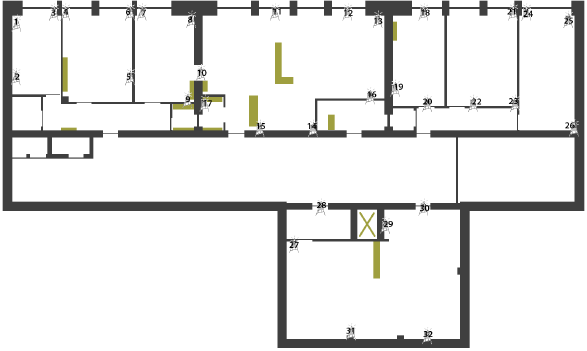
\includegraphics[scale=0.75]{content/images/Testbed}
   	\caption{Floor plan of the area where the Testbed is located. The position of the nodes is shown by the numbered antennas.}
    \label{fig:testbed}
\end{figure}

To monitor the area 32 nodes are distributed over the rooms like shown in Figure \ref{fig:testbed}. The nodes are only placed inside the offices and laboratories and are not always placed at the same hight. To make programming of the devices easy all the devices are connected to Raspberry Pies via USB. A script then makes it possible to copy the source code to all the Raspberry Pies where the code is compiled and then send to each node individual. The connection to the Raspberry Pies makes it also possible to collect information directly from each node individually over serial forwarder running on the Raspberry Pies.

\subsection{TelosB Mote}
The sensor nodes used for the Testbed are Crossbow's TelosB Motes TPR2420. The TPR2420 is a open source platform for researchers developed by the University of California, Berkley. It provides a 8 MHz Texas Instrument MSP430 low power microcontroller with 10kB RAM that is programmable via a USB connector. For communication it includes a IEEE 802.15.4 compliant radio frequency transceiver with an embedded antenna. This makes transmissions in a frequency band from 2.4 to 24835 GHz possible. Moreover the TPR2420 has a light sensor, a Infra-Red sensor, a humidity sensor and a temperature sensor installed making it possible to monitor the environment. Last it has three led lights installed that can be used for visual output of the mote. The USB connector that can be used to program the microcontroller can also be used to exchange data with and to power the TPR2420. If it is not connected via USB it can also be powered by two AA batteries. \cite{telosb}

\begin{figure}[htbp]
	\centering
    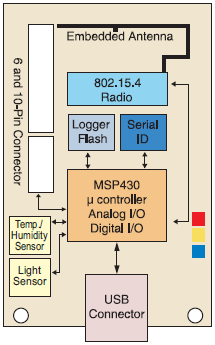
\includegraphics[scale=0.7]{content/images/Mote1}
   	\caption{The structure of the TPR2420 and the included components \cite{telosb}}
    \label{fig:telosb}
\end{figure}
 
\subsection{TinyOs}
TinyOS is an operating system for embedded systems, designed to manage the limited resources and power and to provide reactive concurrency and flexibility. It is widely used by multiple research groups ans companies world wide to support their applications.

The main tasks of TinyOS is to schedule tasks and events to provide safe concurrent operations. However it also provides a large amount of reusable system components, like timers, sender or receiver, that provide a huge variety of functionalities. When compiling a application only the TinyOS components that are used are included into the application creating an application-specific OS.

To provide functionality each component can have three different types of computational abstractions. First there are commands making it possible for other components to call a functionality of the component providing the command. Then there are events which can be signalled by a component. A component receiving the event can than react to it and act accordingly. These two constructs make interaction between components possible. For component intern functionality there are tasks. These can be posted by a component and then will be executed when its their turn. 

Whenever a command, event or task get called it is pushed into the queue of the TinyOS scheduler. The scheduler then executes the tasks inside the queue using a FIFO scheduling policy.    

\subsubsection{Programming for TinyOS}
Applications for TinyOS are written in nesC which us a C dialect and integrates the possibility to implement configurations, modules, interfaces, commands, Events and Tasks. An application consists of components, represented by a nesC module, that provide and use interfaces. The components implement the functionality of the application. All the commands and events a component provides are defined by an interface. Moreover an application for TinyOS also has a configuration that defines which components are connected.   

The Listings \ref{lis:Components}, \ref{lis:interface} and \ref{lis:configuration} show an example application for TinyOS with two components of which one provides an interface and the configuration for the application. This example shows the connections between components, interfaces and the configuration and also shows the use of commands, events and tasks. In Listing \ref{lis:Components} the two components $MainComponent$ and $ExampleC$ are represented. $MainComponent$ uses two interfaces. The first one is the $Boot$ interface. It requires the component to implement the $Boot.booted()$ event. This event is the first event signalled by TinyOS after the node booted. Moreover the $MainComponent$ uses the $ExampleI$ interface that is defined in Listing \ref{lis:interface}. It requires the component to implement the $ExampleI.exampleDone(error_t error)$. The $ExampleI$ interface is provided by the $ExampleC$ component and requires it to implement the $startExample()$ command. Moreover the $ExampleC$ component implements a task $doSomething()$.

Now to connect everything the configuration $Application$ in Listing \ref{lis:configuration} first calls all the components needed for the application. The first component used in this application is the $MainC$ component that provides the $Boot$ interface and is given by TinyOS. Next there are the two components from Listing \ref{lis:Components}. Know the configuration needs to connect the interfaces of the components to the components providing the corresponding interfaces. This means $MainComponent.Boot$ gets connected to $MainC$ and $MainComponent.ExampleI$ gets connected to $ExampleC$.

When a device would get programmed with this example the first thing that would happens is that $MainC$ signals $Boot.booted()$ event resulting in executing the code for the event inside $MainComponent$. This code calls the $ExampleI.startExample$ command. Since the interface is connected to the $ExampleC$ the corresponding code posting the $doSomething()$ task gets executed. Then at the end of $doSomething()$ the $ExampleI.exampleDone(...)$ gets signalled by $ExampleC$. This means the the event gets triggered in $MainComponent$ and the corresponding code gets executed.      

\lstset{caption={Two example components. $MainComponent$ uses the example interface from \ref{lis:interface} and the interface $Boot$ that TinyOS provides. $Boot$ requires the $MainComponent$ to implement the $Boot.booted()$ event that is the first event that gets signalled by TinyOS after the node booted. The $ExampleC$ provides the example interface and therefore needs to implement the event and also implements a task $doSomething()$.},label={lis:Components}}
\begin{lstlisting}
module MainComponent {
	uses interface Boot;
	uses interface ExampleI;
} implementation {
	event void Boot.booted() {
		call ExampleI.startExample();
	}
	
	event void ExampleI.exampleDone(error_t error) {
		if(error == SUCCESS) {
			//some task...
		}
	}
}

module ExampleC {
	provides interface ExampleI;
} implementation {
	task void doSomething() {
		//some task...
		
		signal ExampleI.exampleDone(SUCCESS);
	}
	
	command void startExample() {
		post doSomething();
	}
}
\end{lstlisting}


\lstset{caption={Example interface providing a command $startExample()$ and an event $exampleDone()$.},label={lis:interface}}
\begin{lstlisting}
interface ExampleI {
	command void startExample();
	event void exampleDone(error_t error);
}
\end{lstlisting}

\lstset{caption={The configuration $Application$ links all the Components},label={lis:configuration}}
\begin{lstlisting}
configuration Application {
} implementation {
	components MainC;
	components MainComponent
	components ExampleC;
		
	MainComponent.Boot -> MainC;
	MainComponent.ExampleI -> ExampleC;
}
\end{lstlisting} 

Since whenever a task, command or event gets called it does not get executed directly but gets added to the queue of the TinyOS scheduler. This means that all the tasks, commands or events called before will execute first including the currently running one.  %Materials and Methods
\chapter{Approach}
This chapter explains the general structure and functionality of a system that is supposed to measure the received signal strength of every link in a network.
\TODO Write about what this chapter explains

\section{General Structure}

To measure the RSSI of each link all the nodes need to send messages. Since two nodes sending a message at the same time will distort the RSSI measurements we need to make sure that only one node sends a message at a given point in time. One approach to achieve this is the timeslot based method explained in Chapter 2.3. This method however includes an error inside its timeslots, resulting in a small delay between messages.
To eliminate the delay timeslots bring along a different approach is suggested in this thesis which is based on predefined predecessors for each node. Based on this a node will be able to send a message directly after receiving a message from its predecessor and at the same time making sure that only one node sends at a given point in time.\todo{Complex stuff because of not every node hearing the others}

The system consists of a base station with high processing power and a large memory as well as multiple distributed low power nodes. One of the nodes is the sink which is directly connected to the base station. The nodes are able to communicate with each other via radio, however not every node can hear all the other nodes. This structure is represented by Figure \ref{fig:architecture}. The fact that not every node is able to hear all the other nodes makes it a challenge to collect data from the network and to create a fitting schedule that defines predecessors for all the nodes inside the network. To be able to do so a first calibration phase is needed to create paths from every node to the sink and collect information about the connections between nodes. Then the information about the connections need to be collected at the sink and sent to the base station in a collection phase. When the base station received all the information it can create the schedule. After that the base station has to send the schedule to the sink that starts spreading it inside the network. 

Is the schedule spread and all the nodes know when to send their messages, the sampling of the RSSI can start. Therefore messages are sent according to the predecessors defined in the schedule. All the nodes receiving the messages are now able to measure the received signal strength to the sending node and store this information. When the schedule is completed another collection of the data is needed to gather the measured RSSI at the base station for further processing. When the collection is done, the system can start sampling again and then again collect the data until the system is stopped. This process is shown in Figure \ref{fig:processes}.    

\begin{figure}[htbp]
	\centering
	\begin{subfigure}[t]{0.4\textwidth}
		\centering
    		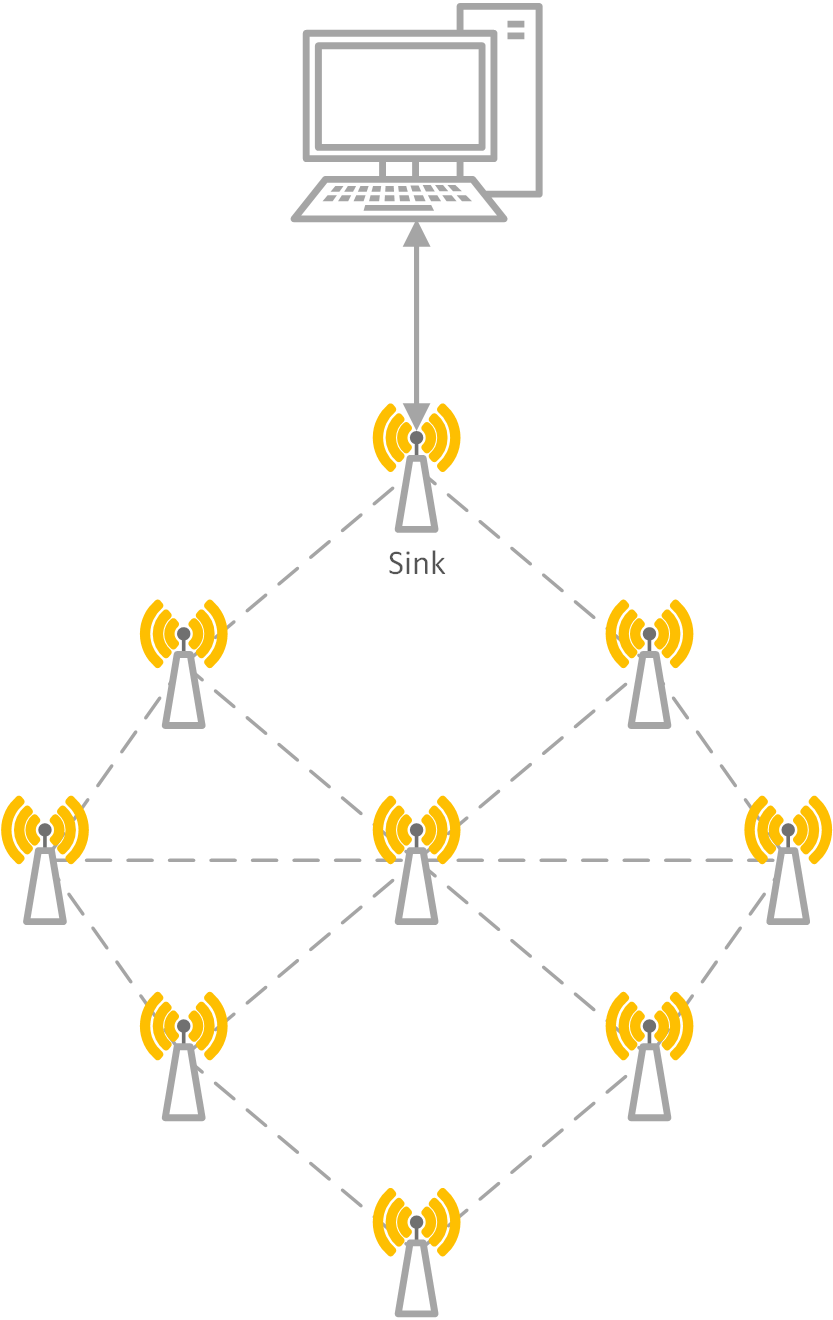
\includegraphics[scale=0.6]{content/images/Architecture}
   	 	\caption{The physical architecture of the system}
    	\label{fig:architecture}
    \end{subfigure}
    \quad
    \quad
    \quad
    \begin{subfigure}[t]{0.4\textwidth}
		\centering         
        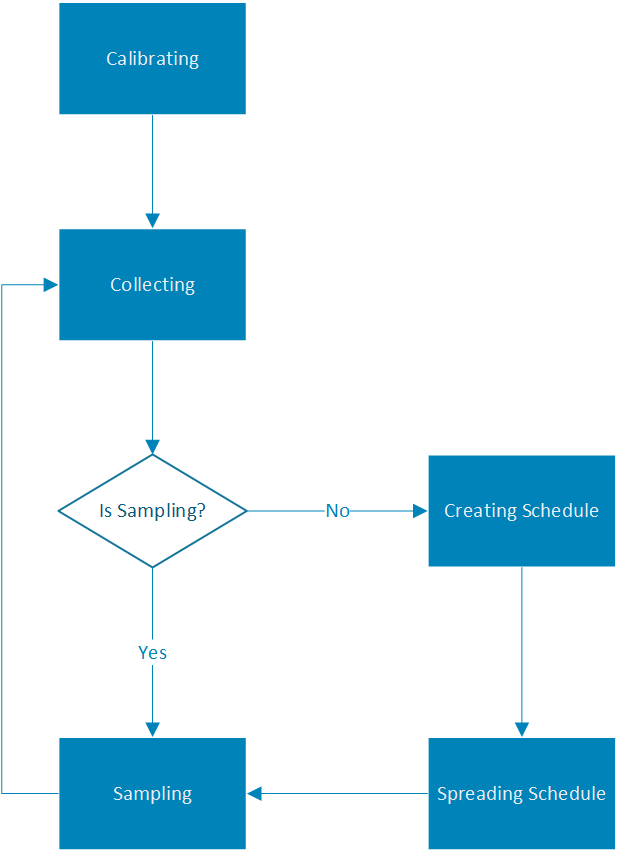
\includegraphics[scale=0.7]{content/images/GeneralAproachM}
        \caption{The general processes and the order in which they are executed}
        \label{fig:processes}
    \end{subfigure}
    \caption{}
\end{figure}

\section{Base Station}
Since creating the schedule and storing and processing the data need a lot of processing power and storage, a base station is needed that fulfils these requirements. This base station needs to be connected to the sink so it can receive the collected data to process it. It also needs to be able to send data to the sink, so the schedule can be spread inside the network. \todo{kill this section?}
  
\section{Calibration}
The calibration has two tasks. It needs to figure out for each node individually which nodes a node has in its range and it needs to create paths to the sink. These paths will then later be used to send data to the sink or spread information inside the network. To achieve these tasks each node will send multiple messages without any specific pattern. \todo{define no pattern}

Each node needs to be able to keep track of the nodes in range. Therefore each node needs to have its own neighbour table. When a node receives a message it can put the node it received the message from inside that neighbour table. All the neighbour tables will later be the basis to create the schedule.

To later collect data from each individual node at the sink, each node needs to know to which node it needs to send its data to so it will reach the sink. This node is the parent of the node. Moreover to spread data inside the network each node also needs to know which nodes will send to itself in direction of the sink. These nodes are the children of a node. When each node found its parent and its children all the paths together will form a tree structure with the sink as the root.

To find the parents for the nodes each node needs to save one extra information and also include this information inside the messages it sends. This information is the quality of the current path a node has to the sink. At the beginning all the nodes except the sink will initialize their path quality with the worst possible value. The sink will initialize its path quality with the best possible value. Now when a node receives a message it will add to the received path quality of the sending node the quality of the link between itself and the sending node to calculate the path quality to the sink for the node, if it would choose the sending node as its parent. The quality of a link is represented by the received signal strength. When the new path quality is calculated the node compares the calculated value with its current path quality. If the calculated value is better the node will set its parent to the sending node and save the new path quality. 

Now, to not only know the direction to the sink but also the direction going away from the sink the nodes need to find their children. Therefore each node will simply include their own parent inside the message it will send. A receiving node will now check if it is the parent of the sending node. If that is the case the receiving node can save the sending node as a child.       

\section{Collection}

\begin{figure}[htbp]
	\label{fig:coll}
	\centering
	\begin{subfigure}[t]{0.4\textwidth}
		\centering
    		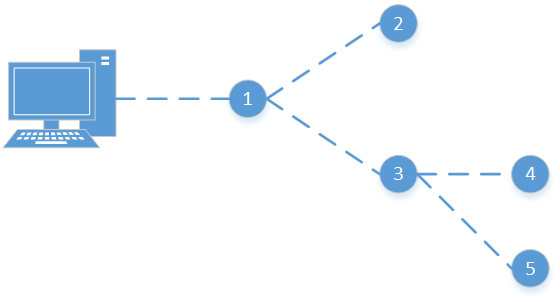
\includegraphics[scale=0.6]{content/images/Collection/Part0}
   	 	\caption{At the beginning all the nodes are unmarked and still have data to send}
    	\label{fig:coll0}
    \end{subfigure}
    \quad
    \quad	
	\begin{subfigure}[t]{0.4\textwidth}
		\centering
    		\includegraphics[scale=0.6]{content/images/Collection/Part1}
   	 	\caption{Node 1 sends the first request to node 2}
    	\label{fig:coll1}
    \end{subfigure}
    \quad
    \quad
    \begin{subfigure}[t]{0.4\textwidth}
		\centering         
        \includegraphics[scale=0.6]{content/images/Collection/Part2}
        \caption{Node 2 does not have any children so it sends its data and gets marked}
        \label{fig:coll2}
    \end{subfigure}
    \quad
    \quad
    \begin{subfigure}[t]{0.4\textwidth}
		\centering         
        \includegraphics[scale=0.6]{content/images/Collection/Part3}
        \caption{Now node 2 is marked so node 1 sends a request to node 3, which forwards it to node 4}
        \label{fig:coll3}
    \end{subfigure}
    \quad
    \quad
    \begin{subfigure}[t]{0.4\textwidth}
		\centering         
        \includegraphics[scale=0.6]{content/images/Collection/Part4}
        \caption{Node 4 does not have any children so it sends its data and gets marked}
        \label{fig:coll4}
    \end{subfigure}
    \quad
    \quad
    \begin{subfigure}[t]{0.4\textwidth}
		\centering         
        \includegraphics[scale=0.6]{content/images/Collection/Part5}
        \caption{Node 3 is still not marked so node 1 sends a request to it. Node 4 is marked so node 3 forwards the request to node 5}
        \label{fig:coll5}
    \end{subfigure}
    \quad
    \quad
    \begin{subfigure}[t]{0.4\textwidth}
		\centering         
        \includegraphics[scale=0.6]{content/images/Collection/Part6}
        \caption{Node 4 does not have any children so it sends its data and gets marked}
        \label{fig:coll6}
    \end{subfigure}
    \quad
    \quad
    \begin{subfigure}[t]{0.4\textwidth}
		\centering         
        \includegraphics[scale=0.6]{content/images/Collection/Part7}
        \caption{Node 3 is still not marked so node 1 sends a request to it}
        \label{fig:coll7}
    \end{subfigure}
    \quad
    \quad
    \begin{subfigure}[t]{0.4\textwidth}
		\centering         
        \includegraphics[scale=0.6]{content/images/Collection/Part8}
        \caption{All the children of node 3 are marked so it starts sending its data and gets marked itself}
        \label{fig:coll8}
    \end{subfigure}
    \quad
    \quad
    \begin{subfigure}[t]{0.4\textwidth}
		\centering         
        \includegraphics[scale=0.6]{content/images/Collection/Part9}
        \caption{Now all the children of node 1 are marked and it can send its own data to the base station and gets marked}
        \label{fig:coll9}
    \end{subfigure}
    \caption{This is an example for the collection. REQ means request and DAT Sx stands for data from source x}
\end{figure}

To collect the data from the network, we make use of the created paths and their tree structure. The process is shown in Figure \ref{fig:coll}. The Figure shows a wireless sensor network represented by the nodes and the paths to the sink created in the calibration phase. Note that the nodes could also have other connections between each other. 

To start the collection the sink sends a request to one of its children. The child receiving that request will check if it has any children himself and if that is the case, it will forward the request to one of them. When the request reaches a node without any children, the node will send its data to its parent which forwards the data to its parent, until the data reaches the sink, which will forward it to the base station. Every node that receives a data message marks the source of that data as done. When the sink sent the received data to the base station, it  sends a new request to one of its children that has not been marked as done. That child again forwards that request to a child that has not been marked as done. If the request reaches a node that has no children or every child has been marked as done it sends its own data. This process will be repeated until the sink does not have any more children left that are not marked as done. Then the sink can send its own data to the base station and finish the collection. All nodes now need to unmark all the other nodes, so another collection is possible.

\section{Creating the Schedule}
Creating a schedule is a quite challenging task since we need an algorithm that visits every node in a graph at least once and starts and ends at the same node. The optimal schedule would be a Hamilton-Circle that is a circle inside a graph that visits each node exactly once. To figure out if a Hamilton-Circle exists, there is however only the way to bruteforce all the possible combinations. This is highly inefficient and possibly we do not even get a result at the end. Therefore this thesis suggests a simple method that makes sure every node gets visited at least once and the path starts and ends at the same node. This method however is not able to create an optimal path and could be improved.

\subsection{Rooted Circles}
\begin{figure}[htbp]
	\centering
	\begin{subfigure}[t]{0.4\textwidth}
		\centering
    		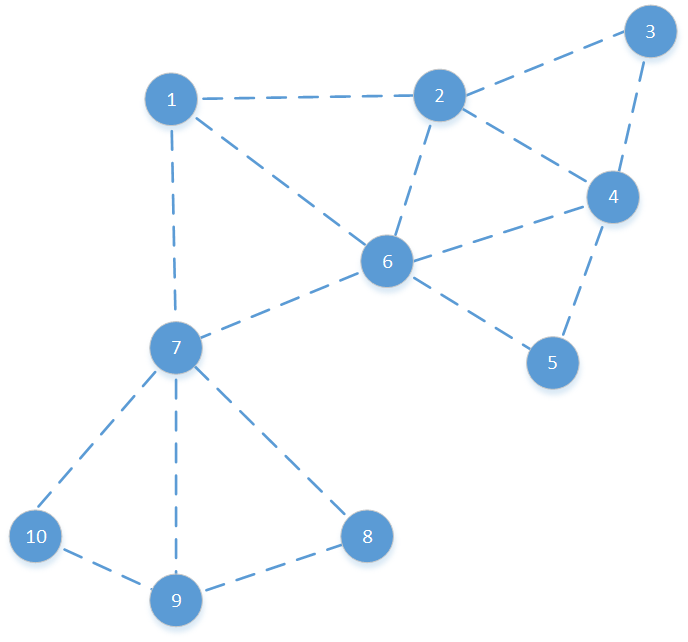
\includegraphics[scale=0.6]{content/images/Schedule/Network}
   	 	\caption{The example network with all its connections between nodes}
    	\label{fig:network}
    \end{subfigure}
    \quad
    \quad
    \begin{subfigure}[t]{0.4\textwidth}
		\centering         
        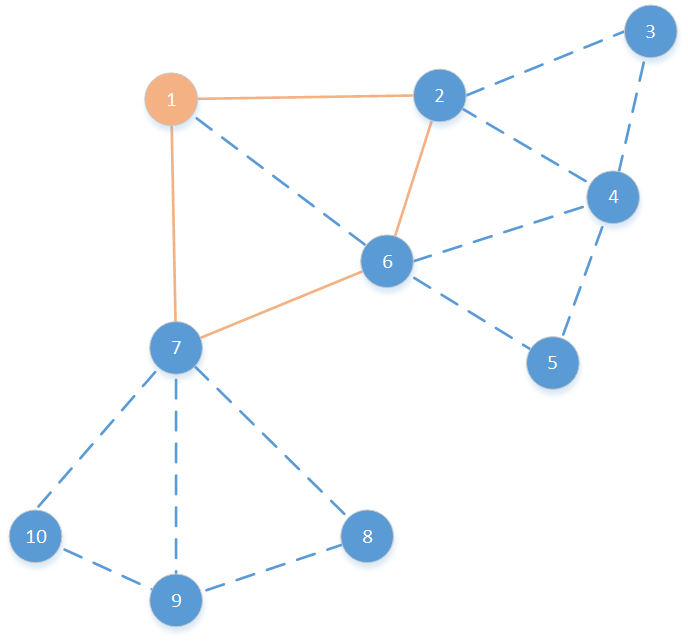
\includegraphics[scale=0.6]{content/images/Schedule/RootedCircle}
        \caption{Example for a rooted circle with node 1 as the root}
        \label{fig:rootedCircle}
    \end{subfigure}
    \label{fig:networkRootedCircle}
    \caption{A rooted circle inside a example network}
\end{figure}

The suggested method is based on smaller circles inside the graph. These circles will have a root node that is the start and the end point of the circle. All the nodes inside this circle will be in range of the root of the circle. These circles will be called rooted circles. In Figure \ref{fig:rootedCircle} such a rooted circle is represented inside the network depicted in Figure \ref{fig:network}. To create a rooted circle, one node needs to be chosen as the root. Then the root will take one node from its neighbour table and choose it as the second node in the circle.  Then the second node will look into its neighbour table and choose a node that has the root node inside its neighbour table. The chosen node will do the same and the process will be repeated until a node does not have a neighbour that has the root as a neighbour. Then the circle will be closed and the path goes to the root. When we look at the example in Figure \ref{fig:rootedCircle} this means node 1 was chosen as the root. Then node 2 was picked as the second node in the circle. Node 2 has multiple neighbours but only one of them, node 6, has the root node 1 as a neighbour. This means node 6 is chosen as the next node in the circle. Node 6 now has node 2 and node 7 as neighbours that also have the root as a neighbour, however node 2 is already inside the circle so node 7 is chosen as the next node. Node 7 now has no more neighbours that have the root as a neighbour and the circle is closed.

\subsection{Creating a Full Schedule}
\begin{figure}[htbp]
	\centering         
    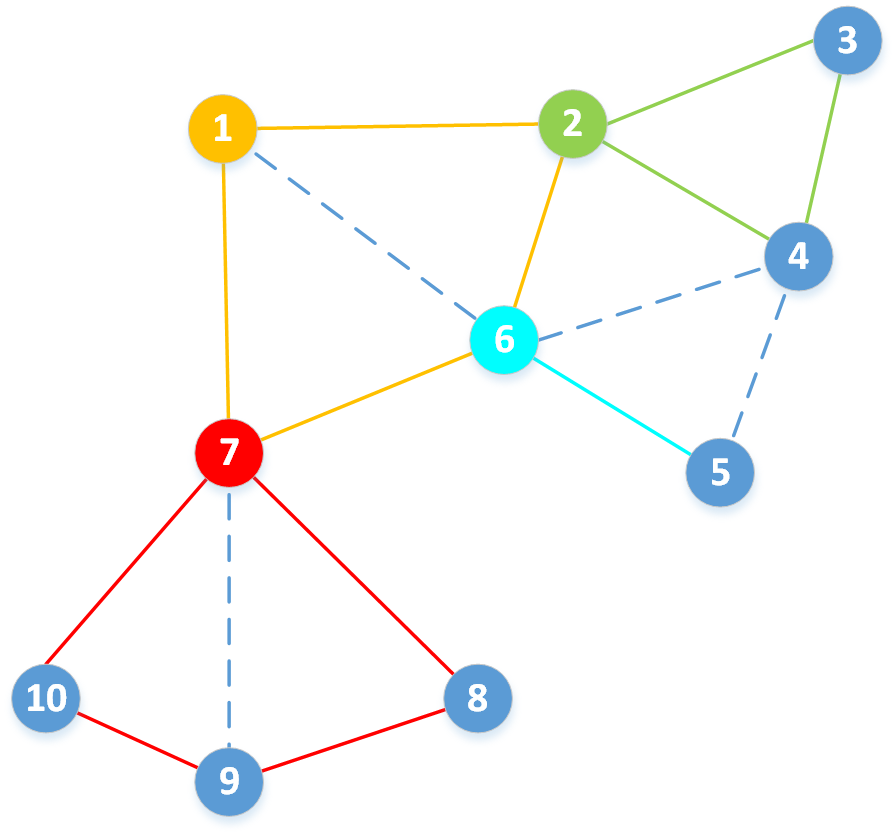
\includegraphics[scale=0.6]{content/images/Schedule/FullSchedule}
    \caption{Full schedule for the example network of Figure \ref{fig:network}. The order in which the nodes send their messages would be: 1 2 3 4 2 6 5 6 7 8 9 10 7 1.}
    \label{fig:schedule}
\end{figure} 
We now want to fill the whole graph with rooted circles. Therefore we will choose the sink as the first root and create a rooted circle around it. When the circle is done, we will go through all the nodes of the circle and, if possible, create rooted circles around them as well. Then we do the same for all the new circles until every node was suggested as a root once. When creating new circles it is not possible to choose a node already inside another circle to be part of the new circle. In Figure \ref{fig:schedule} the network from Figure \ref{fig:network} is fully covered by rooted circles. The first circle created was the one that has node 1 as a root. Then all the nodes inside that circle where chosen as new roots to create new rooted circles. The first thing one could notice is that the circle with the root 6 only has one other node and does not really form a circle. This happens if the circle is closed directly after the second node following the root is chosen because there are no more neighbours left that also have the root as a neighbour. When running the schedule, this means a message would be sent from node 6 to node 5 and then from node 5 back to node 6. Also note that in theory there is a bigger rooted circle possible with the root 6 when node 4 would be included, but node 2 created its rooted circle first and included node 4 and therefore blocked it for rooted circles created at a later point in time. In Listing 3.1 the pseudocode that represents an algorithm to cover a whole graph with rooted circles is shown.

\lstset{caption={Pseudocode that covers a graph with rooted circles},label={lis:rooted}}
\begin{lstlisting}
RootedCircle createRootedCircle(Node root) {
	Node node = getNextForCircle(root, root)	

	If(node != null) {
		RootedCircle rootedCircle = new rootedCircle(root)
		rootedCircle.addNode(node)
		node.setPartOfCircle(true)

		while((node = getNextForCircle(root, node, rootedCircle)) != null) {
			rootedCircle.add(node)
			node.setPartOfCircle(true)
		}

		return rootedCircle
	} else {
		return null
	}
}

Node getNextForCircle(Node root, Node neighbour) {
	for each (Node node in root.getNeighbourList)	
		if(node.isNeighbourOf(neighbour) and not node.isPartOfACircle())
			return node
	return null
}

List<RootedCircle> coverGraphWithRootedCircles(Node firstRoot) {
	List<RootedCircle> circleList = new List<RootedCircle()>
	
	circleList.add(createRootedCircle(firstRoot))

	for each (RootedCircle circle in circleList) {
		for each (Node node in circle) {
			RootedCircle newCircle = createRootedCircle(node)
			if(newCircle != null)
				circleList.add(newCircle);
		}
	}
}
\end{lstlisting}

\section{Spreading the Schedule}
To spread the schedule we will again make use of the tree structure of the created path. When the sink received the schedule from the base station it will forward it to its first child. The child will forward it to one of his children and so on. When a node that received the schedule has no more children, it will send the schedule back to its parent. The parent receiving the schedule will now forward the schedule to its next child. If a parent received the schedule back from all its children, it will forward it to its own parent. In Figure \ref{fig:spreading} an example for this process is given. The Figure shows a wireless sensor network represented by the nodes and the paths to the sink created in the calibration phase. Note that the nodes could also have other connections between each other. 

When you look at the example, one can see that already in Figure \ref{fig:spreading7} the schedule is received by all the nodes but still there are messages sent that could seem useless at this point. However at this point in time we do not know if the sink has any more children that did not receive the schedule yet. Therefore the schedule needs to travel all the way back to the sink. Only at the moment the schedule reaches the sink and the sink does not have any more children left that need to receive the schedule, we know for sure that the schedule is fully spread.

\begin{figure}[htbp]
	\centering
	\begin{subfigure}[t]{0.4\textwidth}
		\centering
    		\includegraphics[scale=0.6]{content/images/ScheduleSpreading/Part1}
   	 	\caption{The base station sends the schedule to node 1.}
    	\label{fig:spreading1}
    \end{subfigure}
    \quad
    \quad
    \begin{subfigure}[t]{0.4\textwidth}
		\centering         
        \includegraphics[scale=0.6]{content/images/ScheduleSpreading/Part2}
        \caption{Node 1 forwards the schedule to node 2}
        \label{fig:spreading2}
    \end{subfigure}
    \quad
    \quad
    \begin{subfigure}[t]{0.4\textwidth}
		\centering         
        \includegraphics[scale=0.6]{content/images/ScheduleSpreading/Part3}
        \caption{Node 2 does not have any children and sends the schedule to its parent node 1}
        \label{fig:spreading3}
    \end{subfigure}
    \quad
    \quad
    \begin{subfigure}[t]{0.4\textwidth}
		\centering         
        \includegraphics[scale=0.6]{content/images/ScheduleSpreading/Part4}
        \caption{Node 2 is now marked so node 1 will forward the schedule to node 3}
        \label{fig:spreading4}
    \end{subfigure}
    \quad
    \quad
    \begin{subfigure}[t]{0.4\textwidth}
		\centering         
        \includegraphics[scale=0.6]{content/images/ScheduleSpreading/Part5}
        \caption{Node 3 forwards the schedule to node 4}
        \label{fig:spreading5}
    \end{subfigure}
    \quad
    \quad
    \begin{subfigure}[t]{0.4\textwidth}
		\centering         
        \includegraphics[scale=0.6]{content/images/ScheduleSpreading/Part6}
        \caption{Node 4 does not have any children and sends the schedule to its parent node 3}
        \label{fig:spreading6}
    \end{subfigure}
    \quad
    \quad
    \begin{subfigure}[t]{0.4\textwidth}
		\centering         
        \includegraphics[scale=0.6]{content/images/ScheduleSpreading/Part7}
        \caption{Node 3 has still node 5 as an unmarked child and forwards the schedule to it}
        \label{fig:spreading7}
    \end{subfigure}
    \quad
    \quad
    \begin{subfigure}[t]{0.4\textwidth}
		\centering         
        \includegraphics[scale=0.6]{content/images/ScheduleSpreading/Part8}
        \caption{Node 5 does not have any children and sends the schedule to its parent node 3}
        \label{fig:spreading8}
    \end{subfigure}
    \quad
    \quad
    \begin{subfigure}[t]{0.4\textwidth}
		\centering
    		\includegraphics[scale=0.6]{content/images/ScheduleSpreading/Part9}
   	 	\caption{Node 3 has no more unmarked children and sends the schedule to its parent node 1}
    	\label{fig:spreading9}
    \end{subfigure}
    \quad
    \quad	
    \begin{subfigure}[t]{0.4\textwidth}
		\centering         
        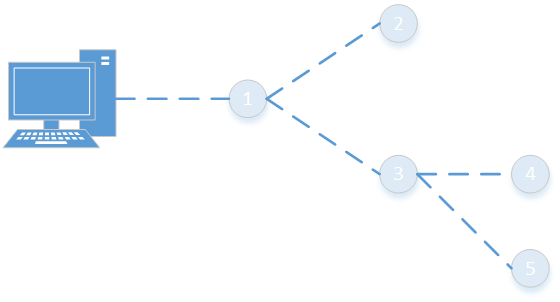
\includegraphics[scale=0.6]{content/images/ScheduleSpreading/Part10}
        \caption{Since node 1 does not have any more unmarked children the schedule is now fully spread inside the network}
        \label{fig:spreading10}
    \end{subfigure}
    \caption{This is an example for a path a schedule message takes to be spread inside the network}
     \label{fig:spreading}
\end{figure}

\section{Sampling}
When all nodes received the schedule it is possible to sample the received signal strength by sending messages according to it. Therefore the sink will start sending a message. When its successor receives the message it can send its message and so on until the last message was send and the sampled data can be collected. However we need to take into account that one node could appear multiple times inside the schedule, meaning a node could have multiple predecessors and successors. Therefore we need to include the successor of the sending node inside the message so a receiving node can see if he is the correct successor at that moment. 
\subsection{Message Drops}
\begin{figure} [htbp]
	\centering         
    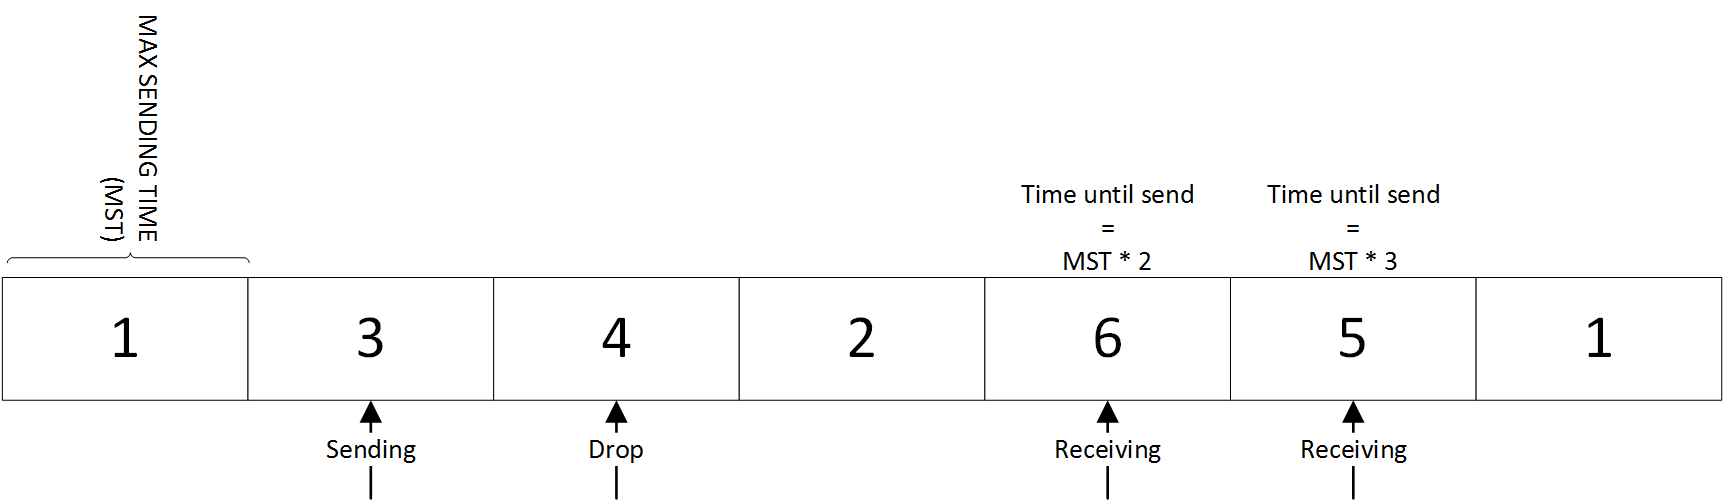
\includegraphics[scale=0.6]{content/images/MessageDrop}
    \caption{Representation of a schedule. Node 3 sends a message. Node 4 drops the message but node 6 and 5 receive it so that they can calculate the time when they should send}
    \label{fig:msgDrop}
\end{figure}
A problem of the proposed method are message drops. If a successor does not receive the message of its predecessor the whole system would stop. Here a similar technique a timeslots based system uses comes in handy. For this method every node needs to know the whole schedule and not only its own predecessors and successors. Then whenever a node receives a message it can look up how many nodes need to send between the node that just send and itself. Than the amount of sending nodes is multiplied by the maximal time a node needs to send a message. The result is the time after the node can send its own message, without receiving a message from its predecessor. Again we need to take into account that a node can appear multiple times in the schedule. Therefore after a node send a message it needs to calculate the maximal time until it will send the next message.

	%Approach
\chapter{Implementation}
\label{chp:imp}

In this chapter a way to implement a system like the one described in Chapter \ref{chp:apr} will be explained by an example based on TinyOS. First it will give you a general overview of the systems structure. Then the individual parts of the system are explained in more detail.    

\section{General Structure}
\label{chp:imp_general}
The system is dividable into two main components. The base station, that stores and processes the data, and the nodes, that collect the data. Both parts of the system need their own hard- and software to complete their tasks.  

\begin{figure}[htbp]
	\centering
    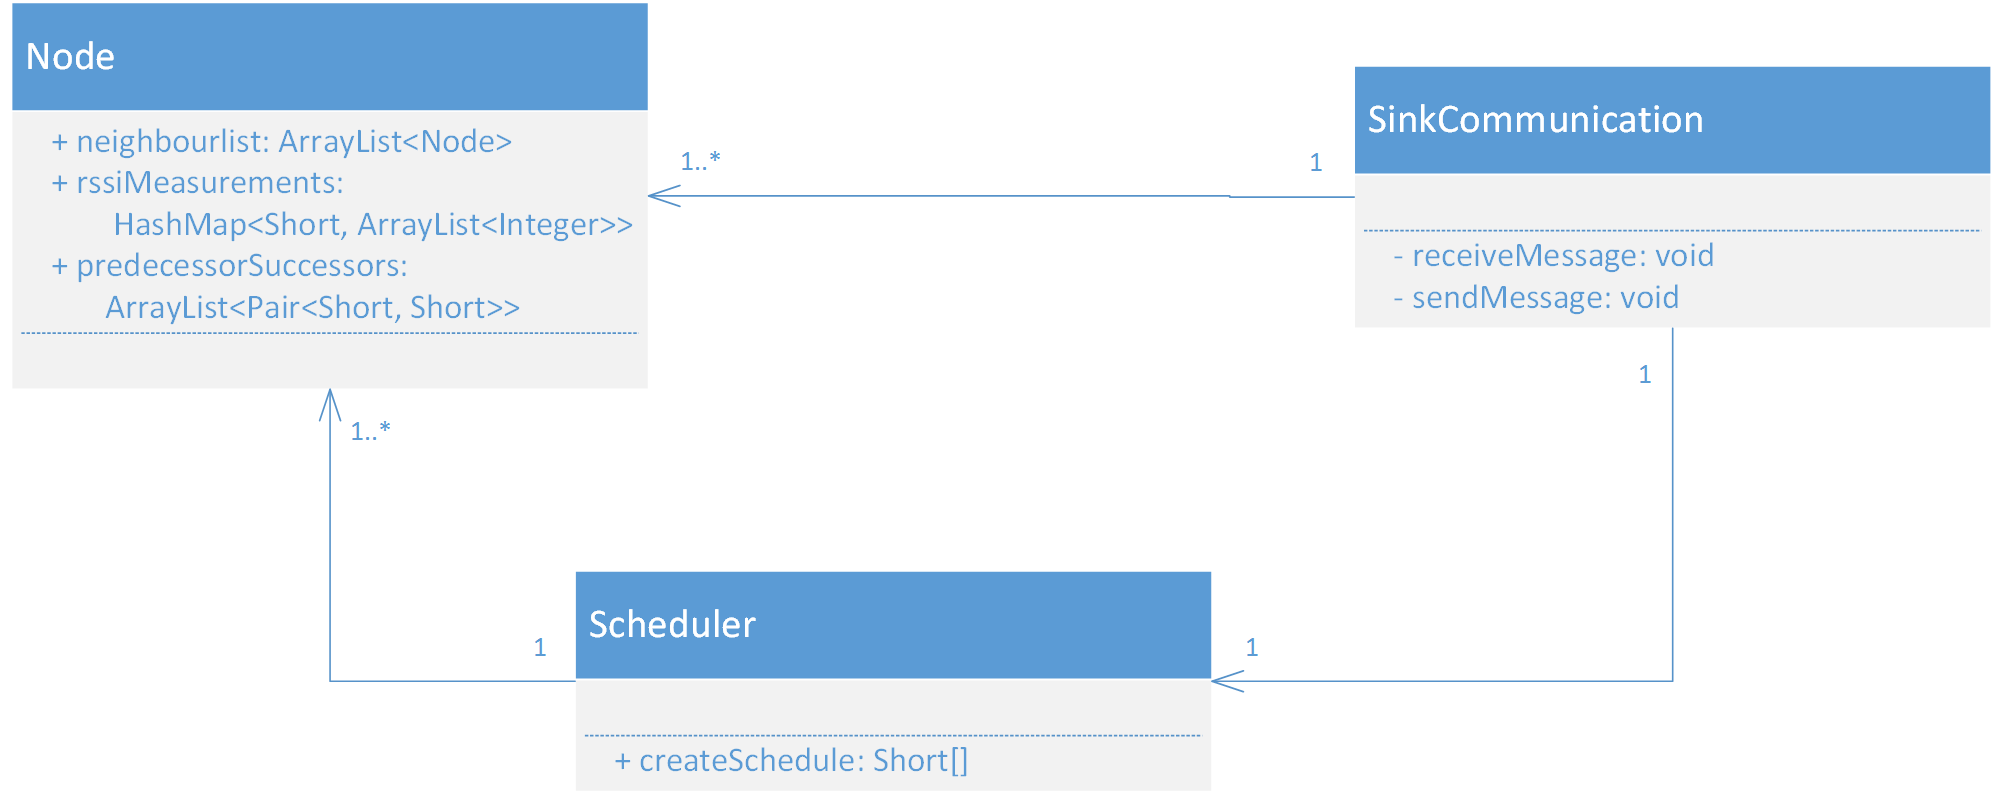
\includegraphics[scale=0.7]{content/images/BaseStation/Klassendiagram}
   	\caption{General structure and functionality of the base station}
    \label{fig:bsKlassen}
\end{figure}

The base station can be a computer running a Java application connected to the sink via a USB-Cable. In Figure \ref{fig:bsKlassen} you can see the general structure of the Java application with its classes and their basic functionality. First, there is the $SinkCommunication$ class that handles the communication with the sink. It is responsible for receiving and processing messages and to send messages to the sink. Then there is the $Node$ class which stores all the information about one node. It stores the neighbours of the node, the measurements a node made and its predecessors and successors. The last class is the Scheduler that is responsible of creating a schedule based on the data saved in the node classes.  

\begin{figure}[htbp]
	\centering
    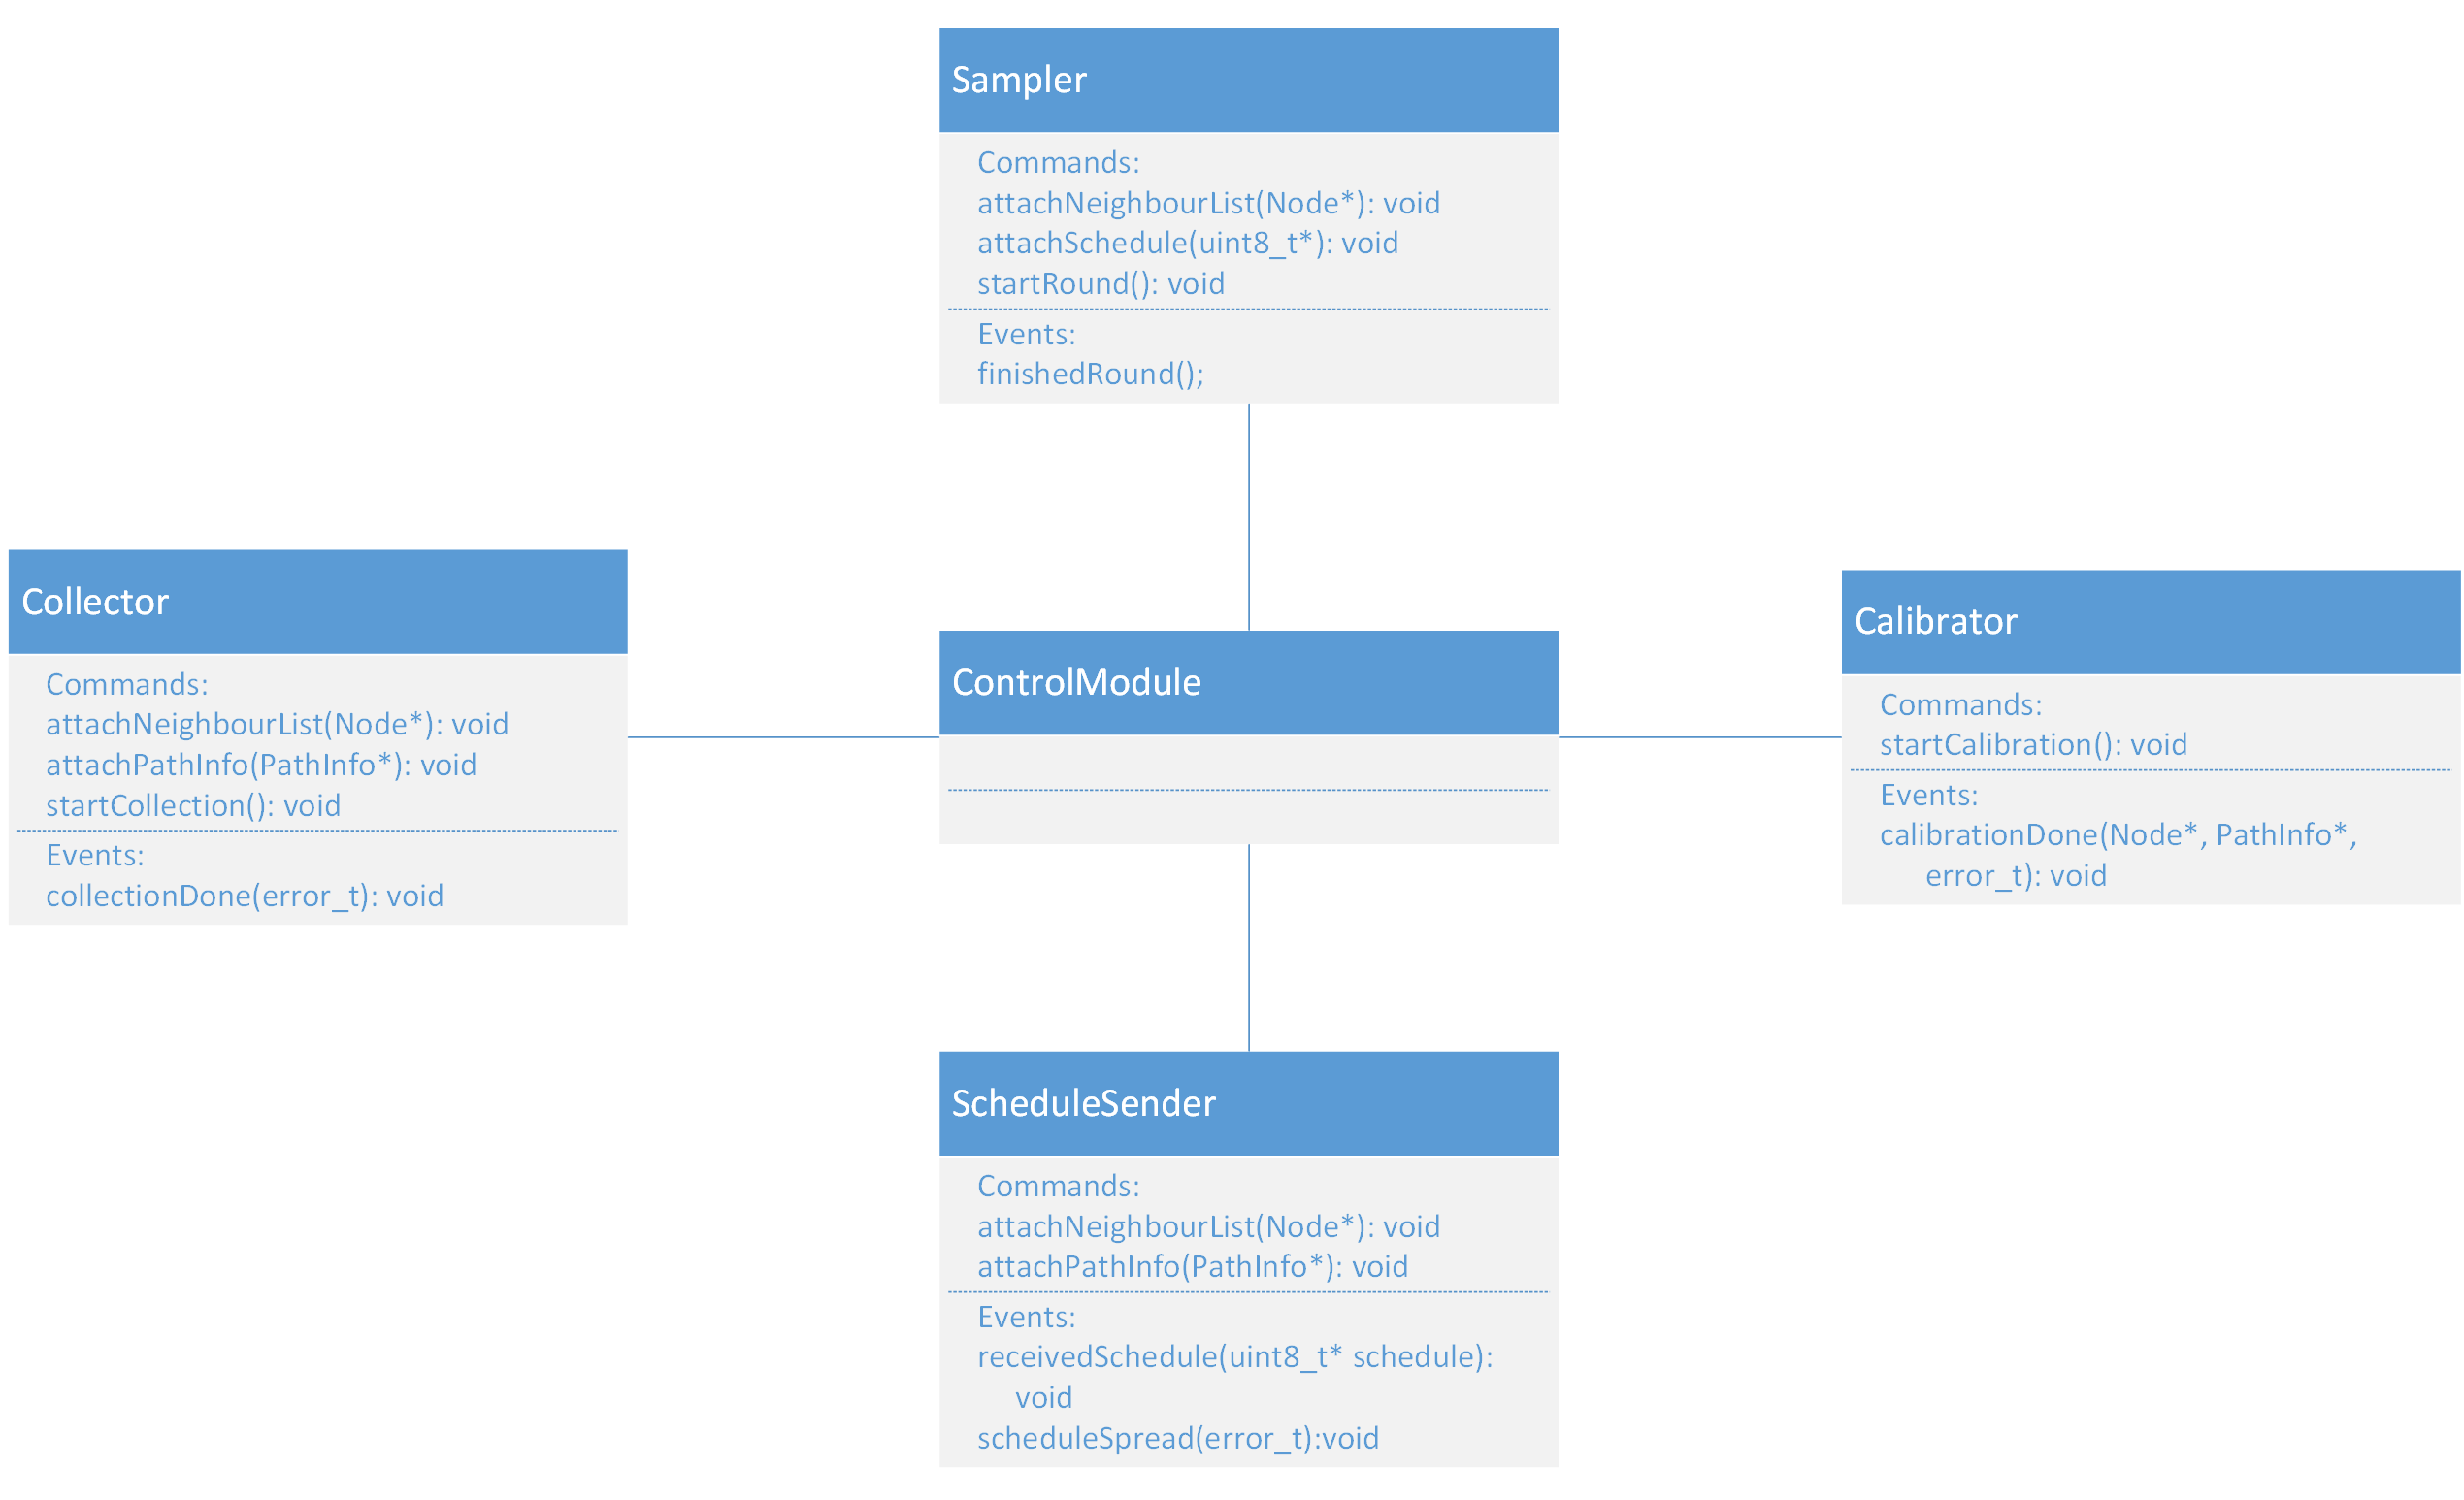
\includegraphics[scale=0.6]{content/images/Motes/GeneralStructure}
   	\caption{The interfaces each module provides. The ControllModule does only use all the other interfaces and does not provide one itself}
    \label{fig:moteStructure}
\end{figure}

\todo{Grafic: attach statt attache und spread statt spreaded, neighbourlist}
As nodes the telosb motes described in Capter x.y can be used. The application running on the nodes can then be written in NESC for TinyOS. Since the application running on the motes has multiple independent tasks it makes to create one module for each task. In Figure \ref{fig:moteStructure} the suggested structure is displayed, containing the modules $Controll$, $Calibrator$, $Sampler$, $ScheduleSender$ and $Collector$" represented by their provided interfaces. 

The $Control$ connects all the other modules and makes sure the informations the other modules provide get delivered correctly to the modules needing that informations. Therefore it does not need an interface to provide functionality.     
The $Calibrator$ module is responsible for the calibration of the network. It has the $startCalibration$ command to start the calibration and the $calibrationDone$ event that gets signalled when the calibration is done and provides the gathered informations. The $Collector$ module covers the data collection. This module needs to know the neighbours and the information about the nodes parent and children. Therefore the interface of the module provides the two commands $attacheNeighbourList$ and $attachePathInfo$ to attach this information to the module. The $Control$ module can then simply attach the information to the $Collector$ when the $calibrationDone$ event triggers. Moreover the $Collector$ module needs the event $collectionDone$ the signal when the collection is done. To spread the schedule inside the network there the application provides the $ScheduleSender$ module. It also needs the information about the neighbours and the parent and children of the node and therefore has the same commands as the $Collector$ to attach these informations. It does not necessary need a command to start the spreading since it can directly react when the node receives a schedule message from the base station. Lastly the module has two events $receivedSchedule$ and $scheduleSpred$. The module signals the $receivedSchedule$ when the node received the schedule and also provides the schedule. When the schedule is spread the sink signals the $scheduleSpread$ event. The last module is the $Sampler$. It needs the neighbour list and the schedule and therefore has the commands $attcheNodeList$ and $attacheSchedule$ to provide these to the module. Moreover it has the $startRound$ command to start one round of the schedule and the $finishedRound$ event that the module signals when this round is finished. Figure \ref{fig:commandEvents} represents a possible sequence of the commands and events.

\begin{figure}[btp]
	\centering
    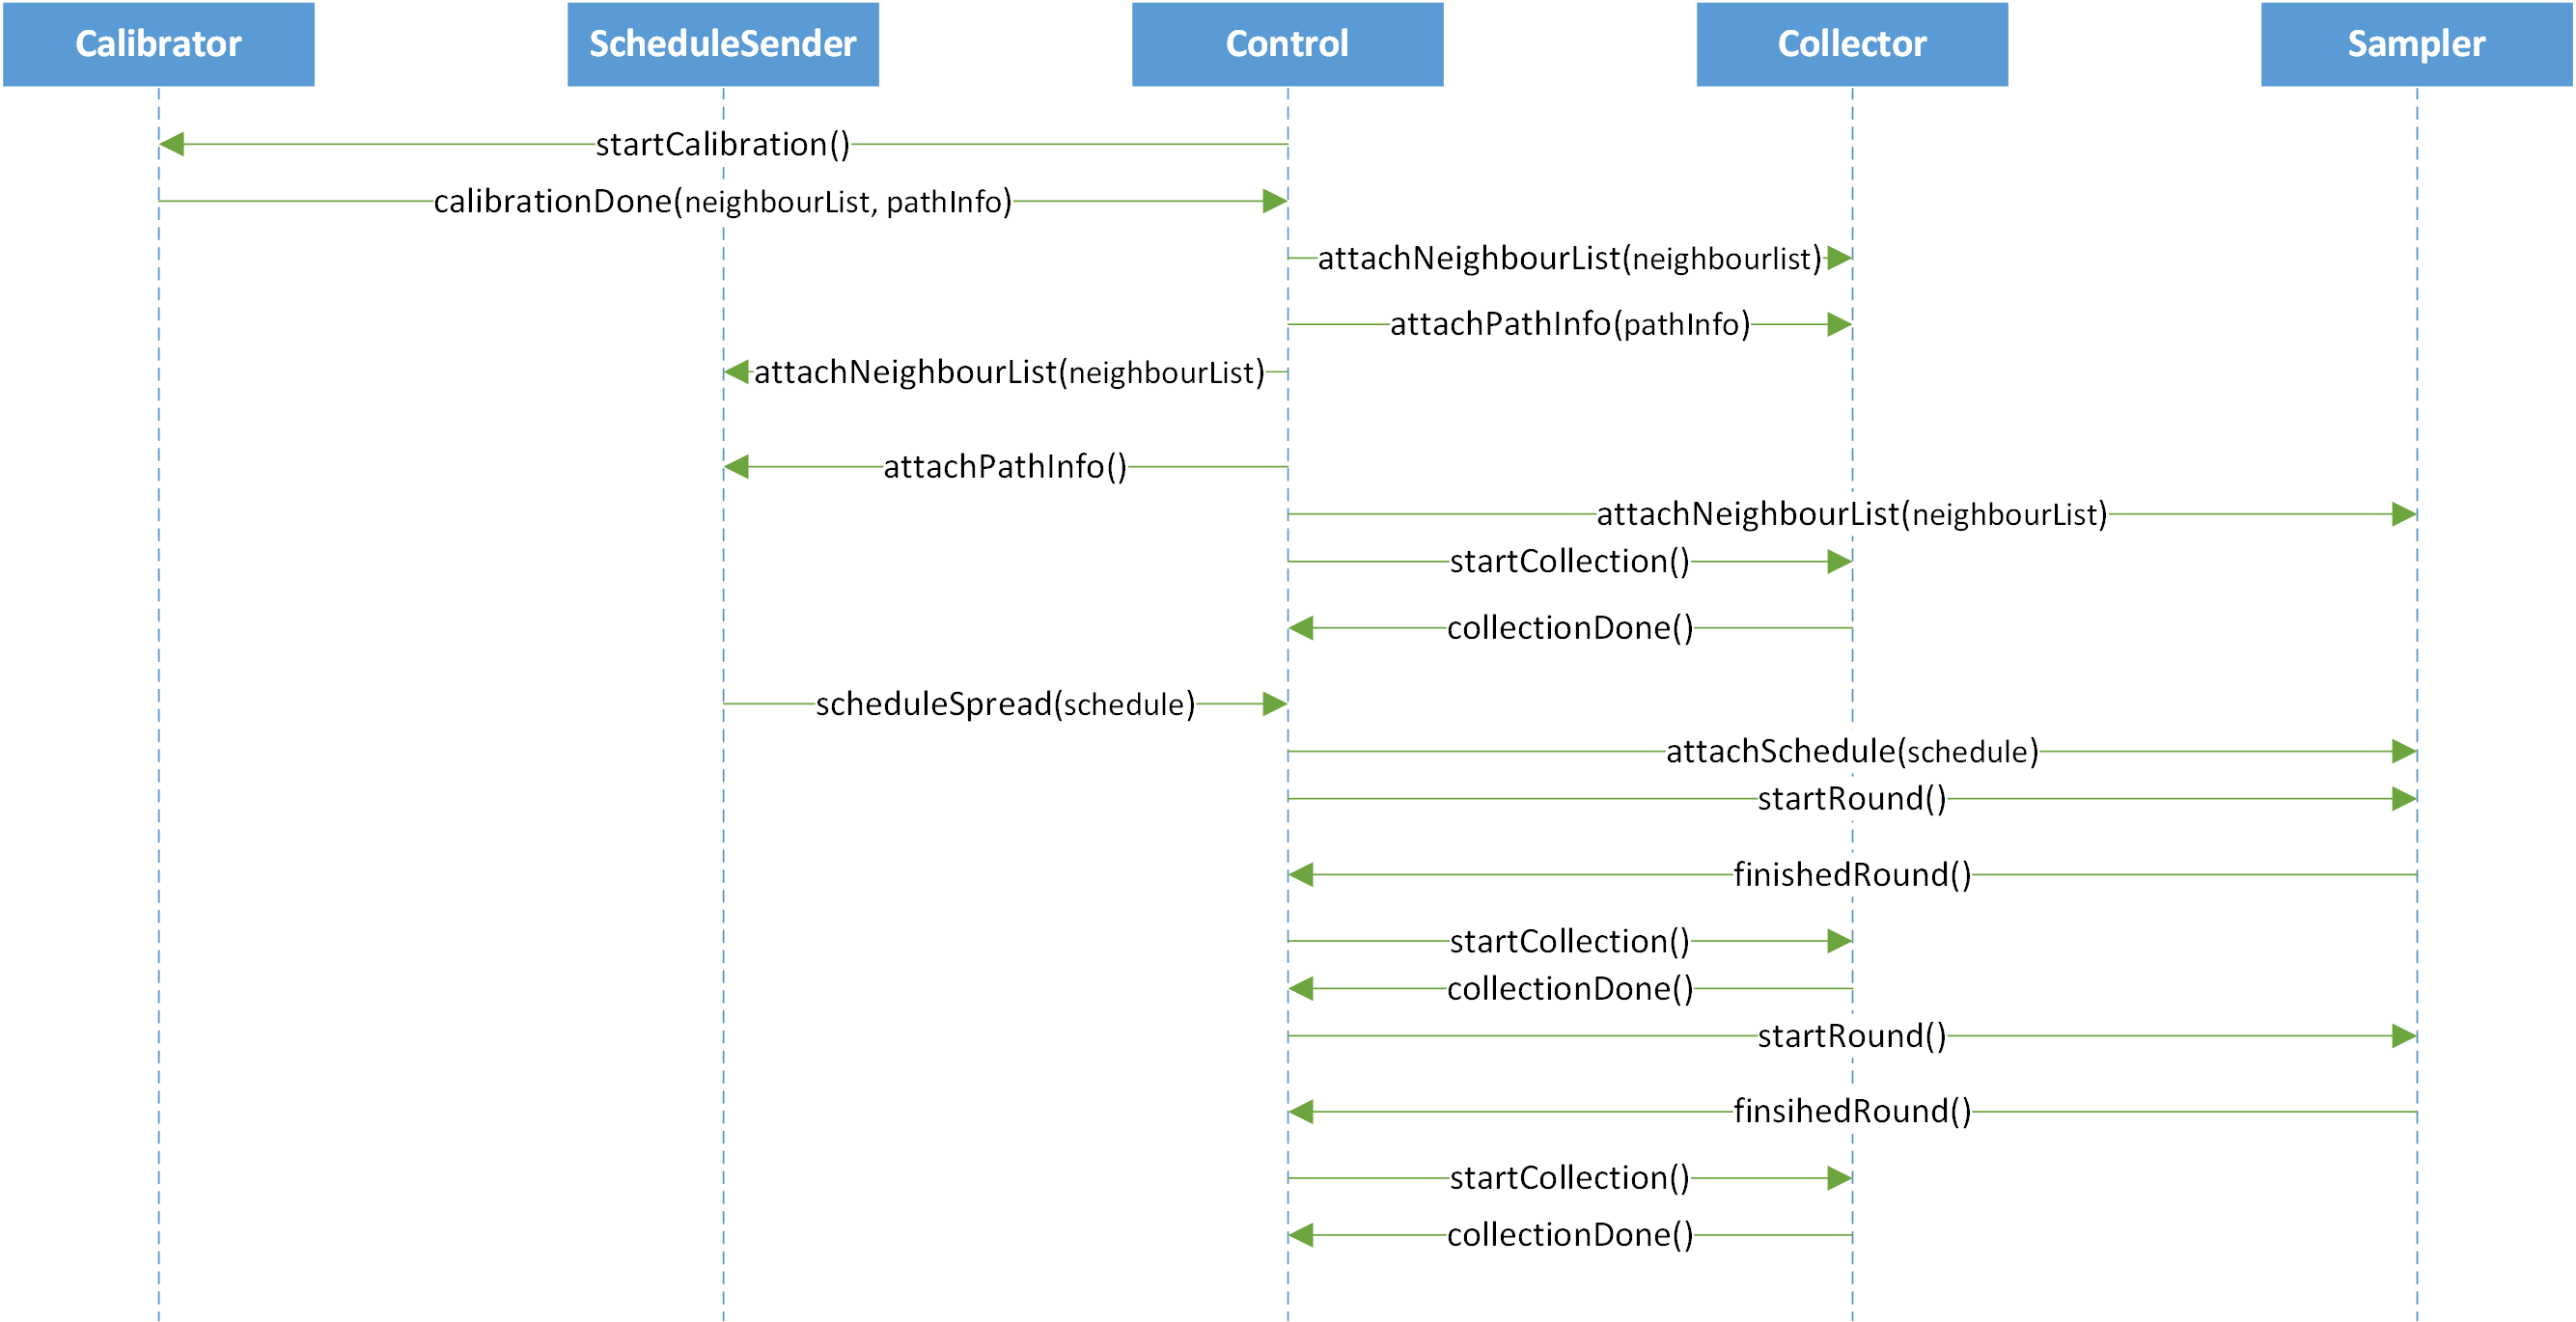
\includegraphics[scale=0.55]{content/images/Processes/ComandsEvents}
   	\caption{A possible order of commands and events.}
    \label{fig:commandEvents}
\end{figure}

\section{Receiving and Storing Information at the Base Station}
\label{chp:imp_baseStation}
To receive and send messages from the sink it is possible to use of the TinyOS Java libraries. These provide the necessary tools to connect the application with the sink via a serial forwarder. To synchronize the message types send by the motes and the Java application TinyOS provides the possibility to generate message classes directly from the NESC message structures. The Java application needs two know different messages. One that contains the information collected by a node and one that contains the information about the schedule. The application know needs to implement message listener for both types of messages so it is able to receive and react to each message individually.

To store information about all the nodes the Java application needs to implement a hash map containing one $Node$ object for every node inside the network with its id as the key. This makes it easy to access the information of each individual $Node$ object when accessing its information. To store the information about a nodes neighbours, the $Node$ class implements a list containing references to $Node$ objects representing the neighbours of the node. To store the RSSI measurements of a node the $Node$ class implements a hash map containing lists. Again the key values of the hash map are node ids. The lists inside the hash map contain all the measurements from the node corresponding to the key. 

Now whenever the Java application receives a message containing measurements of a node it will get the corresponding node object from the hash map containing all the nodes. Then it will update the neighbour list of the node and save the measurements inside the measurement hash map of the node object.
\section{Calibration}
\label{chp:imp_calibration}
To calibrate the the network by using the procedure explained in Chapter \ref{chp:apr_calibration} the Calibration module needs to send messages without a specific pattern. These messages need to contain information about the path quality and the parent of the node. A possible message structure that fulfils these requirements is shown in Listing \ref{lis:callMsg}. 

\lstset{caption={Message structure for the messages, containing information about the parent and the path quality of the sending node},label={lis:callMsg}}
\begin{lstlisting}
	nx_struct CallibrationMsg {
		uint8_t parent,
		uint8_t path_quality
	}
\end{lstlisting}

To make sure that all the node send their messages roughly in the same time interval a way to indicate when the calibration starts is needed. This can be archived by one node starting its calibration phase and the sending of messages. Then when another node receives a $CallibrationMsg$ and hasn't started its calibration it will start its calibration. Another problem is that if all the nodes send their messages directly after another there would be a lot of messages in the network at the same time. To reduce this each node will have a small delay between the messages it will send. To make this even more sufficient each node could have a a different delay between his messages. This delay can be calculated as  
\[ \Delta p = T + \mbox{ID}^2\ \%\ N\]
where $T$ is the minimal time between sends, ID is the nodes id, and $N$ the number of nodes in the whole network. Now whenever a node send a message it can start a timer that fires after $\Delta p$ and then send the next message when the timer fires. Whenever a node sends a message it includes its stored parent and path quality.  

To collect data from other nodes each node needs a neighbour list where it can store the nodes in range and the measured values. This neighbour list can be implemented by an array of the $Node$ struct shown in Listing \ref{lis:nodeStr} and the size $N$. The structure can store the last received signal strength, if the node is in range and the parent of the node. The other fields are used for the other phases. Now whenever a node receives a message it will firstly set the $inRange$ field for that node to $true$, store the measured received signal strength in the $last_rssi$ field and set the $parent$ field to the $parent$ field inside the message. 
 
\lstset{caption={Structure to store information about nodes, containing the last RSSI measured, if the stored node is in range, the parent of the stored node, if the node received the data from stored node, if the node received the schedule from the stored node and the messages received from the stored node},label={lis:nodeStr}}

\begin{lstlisting}
	typedef struct Node {
  		int8_t last_rssi;
  		int8_t inRange;
  		uint8_t parent;
  		int8_t receivedData;
  		int8_t receivedSchedule;
  		uint16_t msg_counter;
	}
\end{lstlisting}

The next thing for the node is to evaluate if it should use the sending node as a parent. This is done like explained in Chapter \ref{chp:apr_collection}. However the link quality is not directly presented by the RSSI. Instead the RSSI is mapped to a value where a high RSSI represents a low value and a low RSSI a high value. An example for the mapping of the RSSI to the path quality is given in Table \ref{tab:mappingRSSI}. This mapping is determined by the network and needs do defined for each individually.
\begin{table}[htbp]
 \caption{Example mapping of RSSI to a value representing the path quality}
 \centering
 \begin{tabular}{c|c}
  RSSI & Quality\\ \toprule
  -50 & 1 \\
  -70 & 2 \\
  -80 & 7 \\
  -90 & 14 \\
 \end{tabular}
 \label{tab:mappingRSSI}
\end{table}
When the link quality is mapped it is added to the $path_quality$ field stored in the message. Than the calculated value is compared to the stored path quality of the sending node. If the calculated value is smaller than the stored path quality the sending node is a more suitable parent and the stored parent and path quality will be adjusted accordingly.   

A node concludes its calibration phase and signals the $callibrationDone$ event after sending a defined number of messages. This number however is also determined by the network and its complexity.  

To make sure the sink does not start to collect data from the network  before every other node finished its calibration it needs to wait after sending all its messages before it can signal the $callibrationDone$ event. The time the sink needs to wait depends on the number of nodes and the calculation of the break between messages.
 
\section{Collection}
\label{chp:imp_collection}
Before starting the calibration the Calibration module needs the information collected by the Calibration module. When the neighbour list and path info is attached to the module the sink can start the collection by sending a request message like the one in Listing \ref{lis:reqMsg} to one of its children. To find a child a node can go through its neighbour list and simply check if the $parent$ field in the $Node$ struct is set to the ID of the node. When a node receives a request message it will search for a child of itself and forward it like described in Chapter \ref{chp:apr_collection}.

\lstset{caption={Structures representing a request message},label={lis:reqMsg}}
\begin{lstlisting}
	typedef nx_struct RequestMsg {
		nx_uint8_t id;
		nx_uint8_t round;
	}
\end{lstlisting}

When the request reaches a node without any children it will fill its measurements into the $measurements$ field of a data message like the one represented in Listing \ref{lis:dataMsg}.
Since it is possible that a node has more measurements than the maximal amount of data fitting into one message we need the field that indicates how much data is left. If a note has more measurements it will directly fill multiple messages and send them one after another to its parent. The receiving node will buffer all the data messages until it received the message where the $dataLeft$ field is set to zero. Then it will forward all the received messages one after another. Whenever a node received the whole dataset of a node it will mark that node as done sending by simply setting the $receivedData$ filed for the node to true. Note that the receiving node does necessary mark the node it directly received the dataset from but the source of the dataset indicated by the $from$ field inside the data messages.

\lstset{caption={Structures to send the data from a node to the sink. The NodeMsg contains the measurements from one neighbour including the id of the neighbour and the measured RSSI. Inside the DataMsg the source of the measurements, the answered request id and how much data is left is stored},label={lis:dataMsg}}
\begin{lstlisting}
	typedef nx_struct Measurement {
		nx_uint8_t id;
		nx_int8_t rssi;
	}

	typedef nx_struct DataMsg {
		nx_uint8_t from;
		nx_uint8_t request_id;
		nx_uint8_t dataLeft;
		Measurement measurements[MAX__MSG__PAYLOAD - 3];
	}
\end{lstlisting}

A problem that needs to be addressed are message drops. Without detecting a message drop and resending the message afterwards the collection will simply stop if one message does not get received. To detect a message drop each node receiving a message will directly send an acknowledgement to the sending node. This is required for both the request and the data message and will be done before any processing of the message. Now if the sending node did not get an acknowledgement for a message will resend that message. Since not only the actual message can drop but also the acknowledgement, it can happen that a message gets retransmitted one or multiple times although the message was already received and processed at the receiving node. The processing of the same message multiple times however can create chaotic behaviour resulting in the system to stop working and/or messages still being send after the collection is already finished and distorting the RSSI measurements. 

To prevent this each request gets an ID from the sink in ascending order and the round of the collection. Whenever a node send its data it will increase its saved round by one and set the saved request id to zero. When a node receives a request it will check if the round of the request is equals the saved round. If not it will throw away the request. If yes it will check if the id of the request is larger than its saved last request id. Is that the case it will save the received request id and process the request, otherwise it will throw it away. To catch already received data messages we include the request id the data was requested with inside the data message. When a node receives a data message it can then check if the data is corresponding to the request the node send. If that is the case it will also check if the $dataLeft$ field in the message is smaller than than the one in the data message previously received. If that is not the case the data inside that message were already received and the message gets thrown away. 

\section{Creating the Schedule}
The creation o the schedule will happen at the base station when it received the data about the connections between nodes. The method presented in Listing \ref{lis:rooted} could be directly translated into the fitting Java code. To do so another class for the rooted circle needs to be added to the general structure of the application. When implementing the method it is important to take into account that links are not always bidirectional meaning when a node 1 is in the neighbour list of another node 2 this only means that node 2 can receive data from node 1, not that node 1 also receives messages from node 2. This means when we chose a node from a neighbour list this node can never be a successor but only a predecessor of a node. This results in the schedule being created backwards.

Moreover it is a good idea to not simply pick a random node as a predecessor from the neighbour list of a node, but the one with the highest measured RSSI. This will reduce message drops while running the schedule, resulting in less time needed for one round.  

To bring the schedule into a form that is readable for all the nodes an array can be created that contains all the node IDs in the order they send messages. For the example in Figure \ref{fig:schedule} the array could look like this: 
\[ Short[]\ schedule = \{1, 2, 3, 4, 2, 6, 5, 6, 7, 8, 9, 10, 7, 1\}\]     
\section{Spreading the Schedule}
Before the spreading of the schedule can start the $ScheduleSender$ module needs the information collected in the Calibration. If the informations are attached to the module the spreading of the schedule automatically when the base station sends a schedule message like the one in  Listing \ref{lis:scheduleMsg} to the sink. The message the schedule array created by the base station, then the information about how much of the schedule is left and an ID to detect already received messages. When the sink receives the schedule message it will forward it like described in Chapter \ref{chp:apr_spreadingSchedule}.

\lstset{caption={Schedule message structure},label={lis:scheduleMsg}}
\begin{lstlisting}
	typedef nx_struct ScheduleMsg {
		nx_uint8_t msgid;	
		nx_uint8_t dataLeft;
		nx_uint8_t schedule[MAX__MSG__PAYLOAD-2];
	}
\end{lstlisting}

Whenever a node receives a message it will first check if it already received that part of the schedule on the basis of the $dataLeft$ field. If it did not receive that schedule part jet it will copy it to the right place in its own schedule array. Then it marks the node it got the message from and forwards it like described in Chapter \ref{chp:apr_spreadingSchedule}. Lastly it checks if the $dataLeft$ field inside the just forwarded schedule message is equals to zero. If that is the case the module will signal the $receivedSchedule$ event and provide the full schedule array to the $Control$ module.
To make it possible to receive multiple schedule parts it is important that whenever a node sends the schedule to its parent, it needs to unmark all its marked nodes, so if necessary it can later send the next schedule part to them.

If the schedule message reaches the sink and the sink does not have any more unmarked children it will forward the schedule to the base station and unmark all its marked nodes. This way the base station knows ether that the schedule is spread or that it can send the next schedule part that then will be spread the same way as the first one. If the sink send the last part of the schedule to the base station the sink will signal the $scheduleSpread$ event to let the $Control$ module know that every node knows the schedule and the sampling can be started. 

Again we need to make sure that no messages get lost, so in this phase as well each message is directly replied by an acknowledgement message. If the sending node did not get the acknowledgement it will resend its message. To check if a message was already received we have the $msgid$ field in the message. Whenever a node forwards the schedule it will increase this field and save the value. Then when a node receives a message it will check if the $msgid$ is larger as the saved one. If that is the case it is a new message and needs to be processed. Otherwise the message gets thrown away. 
\section{Sampling}
When the schedule is spread and the sample module knows about the schedule and the neighbour list, the sampling can start. The sink will start by sending a  message like the on shown in Listing \ref{lis:sampleMsg} in Broadcast. The $receiver$ field will be set to the node id of the successor of the sink. Then all the nodes receiving the message will measure the received signal strength and save it inside their neighbour lists. Then each node that received the message will compare their own id with the id saved in the $receiver$ field of the message. If they are equal the node will evaluate the fitting successor, save it inside a new message and then also send it in broadcast. When the sink receives a message and does not have another successor it will signal the $finishedRound$ event.

To evaluate the fitting successor the approach coming in mind would be to just go through the schedule array and searching for the sending node followed by the searching nodes id. The successor then would be the node after that. This however is inefficient and unnecessarily stretches the timeslot to catch message drops. Therefore it is suggested to evaluate all the predecessors and successors of a node before the sampling starts by going through the whole schedule once and save them in a structure like the one shown in Listing \ref{lis:scheduleSaving} in the order of appearance. Additionally each node will store the index of the next predecessor successor pair. Then when a node is the successor it can simply check if the predecessor at the saved index is correct and if yes send the new message storing corresponding saved successor and calculate the next index as
\[ I+1 = (I + 1)\%\mbox{numberOfPS}\]      
It can happen that the predecessor at the saved index is corresponding to the sending node. This can happen when a message drops and the node gets skipped.
In that case we have to go to all the predecessor successor pairs to find the right successor and adjust the saved index accordingly. However this is still much more efficient than going through the whole schedule.

\lstset{caption={Sample message structure},label={lis:sampleMsg}}
\begin{lstlisting}
	typedef nx_struct SampleMsg {
		nx_uint8_t receiver;
	}
\end{lstlisting} 

\lstset{caption={Structures to save the successor and predecessors},label={lis:scheduleSaving}}
\begin{lstlisting}
	typedef struct PredecessorSuccessor {
		uint8_t predecessor;
		uint8_t successor;
	}

	typedef struct SchedulePSCollection {
		uint8_t numberOfPS;
		PredecessorSuccessor preSuc[MAX_PREDECESSORS_SUCCESSORS]; 
	}
\end{lstlisting}

To catch the message drops like explained in Chapter \ref{chp:apr_samplingDrops} every time a node receives a message and is not the successor it needs to run through the schedule array and and calculate how many nodes send between the sending node and the receiving node and calculate the time it needs for the schedule to reach the node. Then the node will start a timer that fires after exactly that time. Moreover the node needs to save the successor in case of the drop. The timer will be reset to the new time whenever the node receives a message. When the timer fires the node will simply send a message with the $receiver$ set as the saved successor. Since a node can appear multiple times inside the schedule it also needs to calculate the time to its next send directly after it send a message. If it does appear again in the schedule it will start the timer.   %Implementation
\chapter{Evaluation}

%In this chapter you should describe the previous (if possible) and final experiments performed on the implementation.

%Every single experiment should be explained individually, providing to the reader information about the meaning of the experiment, the expected %(theoretical) results, the final results, the comparison between them and others (if possible) and the conclusions. 

%Each experiment should include a description, covering (when possible) the following information:
%\begin{itemize}
%	\item Significant physical features (obstacles present on the environment, human presence, temperature, humidity, possible noise sources, computational speed of the machine, etc.)
%	\item The precise location of the experiment (latitude and longitude, room number or citation to a description of the used laboratory).
%	\item Sampling design (variable(s) measured, transformation performed to the data, samples collected, replication, comparative with a Ground Truth system, collecting data protocol).
%	\item Analysis design (how the data are processed, statistical procedures used, statistical level to determine significance).
%\end{itemize}
%The provided information should be sufficient to allow other scientists to repeat your experiment in the same conditions. Thus, the use of standard and %well-known equipment could only be represented by a simple sentence, but the non-standard equipment should be described in detail, citing the source %(vendor) and most important characteristics.

%To write it, try to use the third person when describing the experiments and results. Avoid to use first person. Past tense should be the dominant %conjugation (the work is done and was performed in the past).

%Note: Graphics represent really well data, use them! (Matlab or Octave could be useful for that).

\section{Experiment Setup}
To test the suggested approach for a RSS measurement system described in Chapter \ref{chp:apr} the approach was implemented like described in Chapter \ref{chp:imp}. System was then deployed and tested inside the Testbed described in Chapter \ref{chp:mat_testbed}. Two experiments where run. The first one was at night where no one was inside the building where the Testbed is located. The second one was at daytime when there where people where working inside the offices covered by the Testbed and also in the other parts of the building. 

The implemented system still had some bugs that could not be addressed due to lack of time. However these bugs only made the system stop at one point during the collection and did not influence the measured times for the different phases. This made it necessary to start the system multiple times for each experiment. The application was restarted after half an hour to catch stops. This however made it impossible to evaluate how long it takes until a new calibration is needed.

To calibrate the system 700 messages were sent. The timeslot for the drops was defined as 18 ms. This is really big but when running the system inside a simulation it could be measured that the processing and sending of a message took between 5 ms and 16 ms the extra 2 ms cover a possible error while measuring these values.  
\section{Experiment Night}
\begin{table}[htbp]
 \caption{Measured values for each run of the system. CT = Calibration Times; HOP = Number of hops inside the schedule; ST = Spread time; ACT = Average collection time; CSTD = Standard deviation of collection time; CR = Total number of collections; ART = Average round time; RSTD = Standard deviation of round time; RR = Total number of rounds}
 \centering
 \begin{tabular}{c||c|c|c|c|c|c|c|c|c}
  Time & CT & HOP & ST & ACT & CSTD & CR & ART & RSTD & RR\\ \toprule
  02:00 - 02:30 & 65611 & 44 & 784 & 3592 & 267 & 338 & 540 & 55 & 338\\
  02:30 - 03:00 & 64545 & 42 & 842 & 3637 & 280 & 73 & 519 & 38 & 73\\
  03:00 - 03:30 & 64630 & 42 & 767 & 4211 & 444 & 13 & 502 & 32 & 13\\
  03:30 - 04:00 & 64539 & 41 & 740 & 3609 & 300 & 420 & 501 & 62 & 420\\
  04:00 - 04:30 & 64565 & 44 & 804 & 3581 & 245 & 419 & 544 & 51 & 419\\
  04:30 - 05:00 & 64699 & 40 & 756 & 4287 & 343 & 35 & 429 & 48 & 35\\
  05:00 - 05:30 & 64587 & 44 & 787 & 4150 & 343 & 9 & 496 & 23 & 9\\
 \end{tabular}
 \label{tab:NightTable}
\end{table}

\begin{figure}[htbp]
	\centering
	\begin{subfigure}[t]{1\textwidth}
		\centering
    		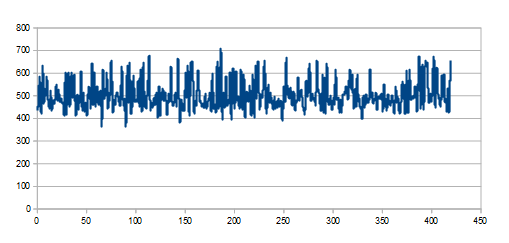
\includegraphics[scale=0.75]{content/images/Experiment/NightRounds}
   	 	\caption{The physical architecture of the system}
    	\label{fig:architecture}
    \end{subfigure}
 
    \begin{subfigure}[t]{1\textwidth}
		\centering         
        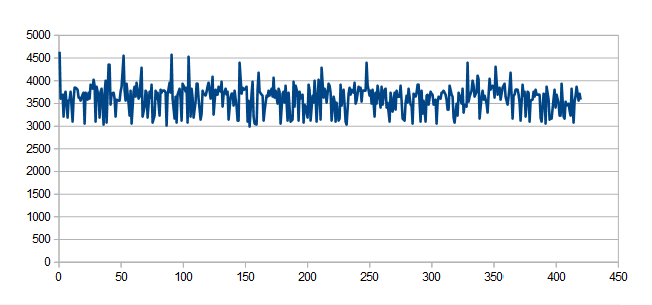
\includegraphics[scale=0.75]{content/images/Experiment/NightCollection}
        \caption{The general processes and the order in which they are executed}
        \label{fig:processes}
    \end{subfigure}
    \caption{}
\end{figure}

\section{Experiment Day}
\begin{table}[htbp]
 \caption{Measured values for each run of the system. CT = Calibration Times; HOP = Number of hops inside the schedule; ST = Spread time; ACT = Average collection time; CSTD = Standard deviation of collection time; CR = Total number of collections; ART = Average round time; RSTD = Standard deviation of round time; RR = Total number of rounds}
 \centering
 \begin{tabular}{c||c|c|c|c|c|c|c|c|c}
  Time & CT & HOP & ST & ACT & CSTD & CR & ART & RSTD & RR\\ \toprule
  09:15 - 09:45 & 64647 & 43 & 823 & 4401 & 296 & 63 & 492 & 41 & 63\\ 
  09:45 - 10:15 & 64558 & 44 & 796 & 4035 & 322 & 121 & 563 & 59 & 121\\
  10:15 - 10:45 & 64644 & 41 & 850 & 3740 & 282 & 231 & 482 & 40 & 231\\
  10:45 - 11:15 & 64577 & 41 & 849 & 3746 & 423 & 14 & 533 & 60 & 14\\ 
  11:15 - 11:45 & 64607 & 39 & 797 & 3498 & 358 & 433 & 495 & 42 & 433\\
  11:45 - 12:15 & 64654 & 41 & 764 & 3556 & 294 & 240 & 495 & 45 & 240\\
  12:15 - 12:45 & 64583 & 44 & 824 & 4160 & 511 & 368 & 539 & 65 & 368\\
  12:45 - 13:15 & 64544 & 44 & 797 & 3697 & 398 & 183 & 542 & 58 & 183\\
  13:15 - 13:45 & 64580 & 41 & 778 & 3494 & 371 & 73 & 528 & 46 & 73\\
 \end{tabular}
 \label{tab:NightTable}
\end{table}

\begin{figure}[htbp]
	\centering
	\begin{subfigure}[t]{1\textwidth}
		\centering
    		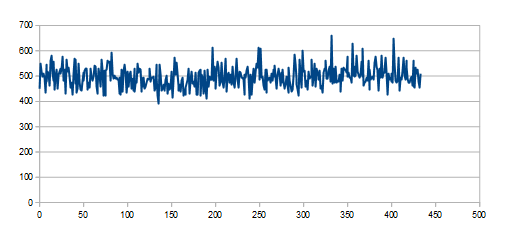
\includegraphics[scale=0.75]{content/images/Experiment/DayRounds}
   	 	\caption{The physical architecture of the system}
    	\label{fig:architecture}
    \end{subfigure}
 
    \begin{subfigure}[t]{1\textwidth}
		\centering         
        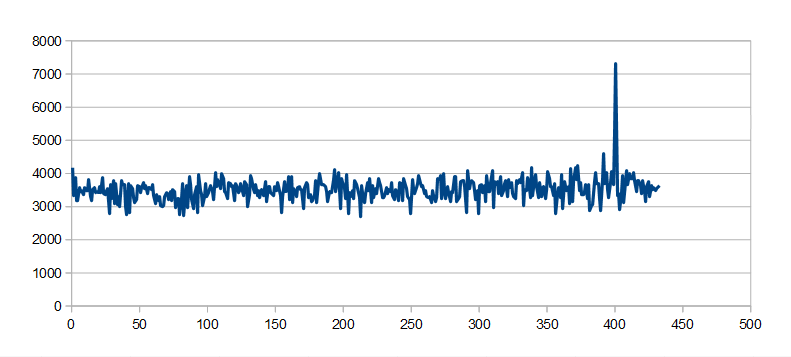
\includegraphics[scale=0.75]{content/images/Experiment/DayCollection}
        \caption{The general processes and the order in which they are executed}
        \label{fig:processes}
    \end{subfigure}
    \caption{}
\end{figure} %Evaluation
\chapter{Discussion}

%The meaning of this paragraph is to interpret the results of the performed work. It will always connect the %introduction, the postulated hypothesis and the results of the thesis/bachelor/master.

%It should answer the following questions:
%\begin{itemize}
%	\item Could your results answer your initial questions?
%	\item Did your results agree with your initial hypothesis?
%	\item Did you close your problem, or there are still things to be solved? If yes, what will you do to %solve them? 
%\end{itemize}

\section{Possible Improvements}
The first improvement for the calibration was already explained. Here time can be saved by simply calculating the correct break and not having the system do nothing for 25 seconds.

The next improvement is for the collection. When using nodes with a lot of memory, it could be a good idea to not always send the data from one node directly to the sink but first collect all the data of a node's children before forwarding it. This way the requests and data messages would take the same path as the schedule while spreading it. This would reduce the amount of requests and the overall collection time.
 
Another improvement can be done to the algorithm that creates the schedule. Instead of just covering the network with rooted circles, it is possible to later connect circles in a way that reduces the amount of messages. Also to improve choosing a next node, it would be a good idea to change the calibration in a way that not only the last measured RSS for each link gets saved but an average RSS for a link.
A different way to maybe improve the schedule is to simply select the same path a schedule message would take while spreading it. The experiments already show that spreading the schedule is faster than the rounds with the created schedule. 

\section{Conclusion}
Because the existing approach for signal strength measurement does not work inside a multi-hop wireless sensor network, a new approach was developed that works for multi-hop WSNs. The new approach consists of different phases. First, there is a calibration phase where information about the network is collected. Moreover, paths through the WSN are created to collect information at a central point and to spread information inside the network. Then in the next phase, a schedule that defines predecessors and successors for each node is created and spread inside the network. Last, the measurement of the signal strength. Therefore each node will send messages according to the schedule, meaning one node starts sending a message. All the nodes hearing that message will measure the signal strength and store it. When a node hears a message from its predecessor, it can send its own message. This goes on until every node sent a message. Then the stored measurements of the nodes are collected at the central point and a new measurement round can begin, enabling the possibility to monitor the signal strength of each link over a period of time.

This approach was implemented and tested in a WSN testbed located at the University of Duisburg-Essen. The experiments show that for a WSN with 32 widely spread nodes one measurement round takes about 500 ms followed by a 3.5 second collection phase. This means that the system can deliver one full set of measurements every four seconds by taking multiple rounds of measurements one after another. This is sufficient to fulfill the requirements of measurements necessary to compute RTI with a person walking in the environment.   	%Discussion
\chapter{Acknowledgements}

(This part is optional, and it could be completely excluded by deleting \\ 
\textbf{ \textbackslash include \{content/chapters/chapter7\}} \\
from the Firstname\_Lastname\_Diplom\_Master\_arbeit.tex file)

This paragraph could mention people or institutions that supported you to some extent with your work or friends and relatives that supported you during your study period. 
	%Aknowledgments


% Appendix chapters to be put here. They will be enumerated with capital letters 
% if you  did not change the \documentclass options.
\begin{appendix}


%\include{appendix_chapterA}
\end{appendix}
%Ende Anhang

%Bibliography
% We strongly recommend to use bibtex to manage your bibliography. It helps you
% structure your references and helps avoiding missing important data for a correct
% quotation. If you have no other idea jabref (http://jabref.sourceforge.net/)
% might be a good idea (Jave runtime environment needed).
% This style is good to use in german master thesis'. You need to have activated
% \usepackage{bigerm} above.
% For english documents just use apalike.
\bibliographystyle{geralpha}


% to finally announce where your bibliography is stored use
\bibliography{content/references/references}
% it is also possible to have several files separated by comma. 
%Bibliographie Angaben mit \bibliography{}

%pagenumbering{null}

\ 

%clearpage
\cleardoublepage

\ 

\pagestyle{empty}
\vfill
\textbf{Erklärung}\\

\[German\] Hiermit versichere ich, dass ich die vorliegende Bachelorarbeit selbständig verfasst, keine anderen als die angegebenen Quellen und Hilfsmittel benutzt, sowie Zitate kenntlich gemacht habe.\\

\[English\] I hereby declare that I have written this Bachelor thesis independently, using no other than the specified sources and resources, and that all quotations have been indicated.\\
\\\\
Essen, \today\\
$\overline{\parbox{3.5cm}{(Place, Date)}} ~~~~~~~~~~~~~~~~~~~~~~~~~~~ \overline{\parbox{4cm}{\studentFirsName { } \studentSecondName}}$
 %It may be necessary that you replace "Bachelorarbeit" with "Masterarbeit" here...

\end{document}
%%% Local Variables:
%%% mode: latex
%%% TeX-master: t
%%% End:
